%!TEX TS-program = xelatex

%!TEX root = ../Thesis.tex

% This information is used in titlepage, colophon, preface and hyperref setup (pdf metainfo), and other options.

\def\thesistypeabbr{MSc}
\def\thesistype{Master of Science}

\def\thesisauthor{Andreas Madsen (s123598)}
\def\thesistitle{Semi-Supervised Neural Machine Translation}
\def\thesissubtitle{for small bilingual datasets}
\def\thesislocation{Kongens Lyngby}
\def\thesisdeadline{June 31, 2017}

\def\papersize{b5paper} % Final papersize (b5paper/a4paper), recommended papersize for DTU Compute is b5paper
\def\showtrims{false} % Print on larger paper than \papersize and show trim marks (true/false)?

%!TEX root = ../Thesis.tex
\newcommand{\papersizeswitch}[3]{\ifnum\strcmp{\papersize}{#1}=0#2\else#3\fi}
\papersizeswitch{b5paper}{\def\classfontsize{10pt}}{\def\classfontsize{12pt}}

\documentclass[\classfontsize,\papersize,twoside,showtrims,openany]{memoir}
\RequireXeTeX
% DOCUMENTATION: https://tug.org/pracjourn/2008-2/madsen/madsen.pdf

\showtrimsoff
\papersizeswitch{b5paper}{
    % Stock and paper layout
    \pagebv
    \setlrmarginsandblock{26mm}{20mm}{*}
    \setulmarginsandblock{35mm}{30mm}{*}
    \setheadfoot{8mm}{10mm}
    \setlength{\headsep}{7mm}
    \setlength{\marginparwidth}{18mm}
    \setlength{\marginparsep}{2mm}
}{
    \papersizeswitch{a4paper}{
        \pageaiv
        \setlength{\trimtop}{0pt}
        \setlength{\trimedge}{\stockwidth}
        \addtolength{\trimedge}{-\paperwidth}
        \settypeblocksize{634pt}{448.13pt}{*}
        \setulmargins{4cm}{*}{*}
        \setlrmargins{*}{*}{0.66}
        \setmarginnotes{17pt}{51pt}{\onelineskip}
        \setheadfoot{\onelineskip}{2\onelineskip}
        \setheaderspaces{*}{2\onelineskip}{*}
    }{
    }
}
\ifnum\strcmp{\showtrims}{true}=0
    % For printing B5 on A4 with trimmarks
    \showtrimson
    \papersizeswitch{b5paper}{\stockaiv}{\stockaiii}
    \setlength{\trimtop}{\stockheight}
    \addtolength{\trimtop}{-\paperheight}
    \setlength{\trimtop}{0.5\trimtop}
    \setlength{\trimedge}{\stockwidth}
    \addtolength{\trimedge}{-\paperwidth}
    \setlength{\trimedge}{0.5\trimedge}
    \trimLmarks
\fi

\checkandfixthelayout                 % Check if errors in paper format!
\sideparmargin{outer}                 % Put sidemargins in outer position
\reversemarginpar			        % Put marginpar in outer position

% Links
\usepackage[hyphens]{url}             % Allow hyphens in URL's
\usepackage[psdextra]{hyperref}       % References package

% Graphics and colors
\usepackage{graphicx}                 % Including graphics and using colours
\usepackage[svgnames]{xcolor}         % Defined more color names
\usepackage{eso-pic}                  % Watermark and other bag
\usepackage{preamble/dtucolors}
\graphicspath{{graphics/}}

% Table of contents (TOC)
\setcounter{tocdepth}{1}              % Depth of table of content
\setcounter{secnumdepth}{2}           % Depth of section numbering

% Paragraph style (no indent and space between pragraphs)
\setlength{\parindent}{0pt}
\setlength{\marginparwidth}{50pt} 
\nonzeroparskip

\newcommand{\marginnote}[1]{\marginpar{\footnotesize{#1}}}

% Definea hrule there doesn't depend on the chars, used in the mychaperstyle  
\newcommand{\HRule}[1][\medskipamount]{\par
  \vspace*{\dimexpr-\parskip-\baselineskip+#1}
  \noindent\rule{\linewidth}{0.2mm}\par
  \vspace*{\dimexpr-\parskip-.5\baselineskip+#1}}

% Chapterstyle
\makeatletter
\makechapterstyle{mychapterstyle}{
    \chapterstyle{default}
    \def\format{\normalfont\sffamily}

    \setlength\beforechapskip{0mm}

    \renewcommand*{\chapnamefont}{\format\LARGE}
    \renewcommand*{\chapnumfont}{\format\fontsize{40}{40}\selectfont}
    \renewcommand*{\chaptitlefont}{\format\fontsize{32}{32}\selectfont}

    \renewcommand*{\printchaptername}{\chapnamefont\MakeUppercase{\@chapapp}}
    \patchcommand{\printchaptername}{\begingroup\color{dtugray}}{\endgroup}
    \renewcommand*{\chapternamenum}{\space\space}
    \patchcommand{\printchapternum}{\begingroup\color{dtured}}{\endgroup}
    \renewcommand*{\printchapternonum}{%
        \vphantom{\printchaptername\chapternamenum\chapnumfont 1}
        \afterchapternum
    }

    \setlength\midchapskip{1ex}

    \renewcommand*{\printchaptertitle}[1]{\raggedleft \chaptitlefont ##1}
    \renewcommand*{\afterchaptertitle}{\vskip0.5\onelineskip \HRule[5pt] \vskip1.3\onelineskip}
}
\makeatother
\chapterstyle{mychapterstyle}

% Section style
\usepackage{titlesec}
\maxsecnumdepth{subsection} % numbering on subsection
\maxtocdepth{subsection}
\titleformat*{\section}{\LARGE\bfseries}
\titleformat*{\subsection}{\Large\bfseries}
\titleformat*{\subsubsection}{\large\bfseries}
\titleformat*{\paragraph}{\large\bfseries}
\titleformat*{\subparagraph}{\large\bfseries}

% header and footer
\setlength{\headwidth}{\textwidth}
\pagestyle{companion}
\aliaspagestyle{chapter}{plain}

% Chapter changes
\newcommand*\cleartoleftpage{%
  \clearpage
  \ifodd\value{page}\hbox{}\newpage\fi
}

% Create a caption box for equations
% http://tex.stackexchange.com/questions/97029/referencing-equation-counter-value-in-custom-float-caption
\usepackage{aliascnt}
\usepackage{float}
\newaliascnt{equationbox}{equation}
\newfloat{equationbox}{h}{Equation}
\floatname{equationbox}{Equation}

% Bold caption labels
\usepackage[labelfont=bf]{caption}
\makeatletter
\renewcommand\@memmain@floats{%
  \counterwithin{equation}{section}
  \counterwithin{equationbox}{section}
  \counterwithin{figure}{section}
  \counterwithin{table}{section}}
\makeatother

% Hypersetup
\hypersetup{
    pdfauthor={\thesisauthor{}},
    pdftitle={\thesistitle{}},
    pdfsubject={\thesissubtitle{}},
    pdfdisplaydoctitle,
    linktoc=all,
    plainpages=false,
    unicode=true,
    bookmarks,
    bookmarksnumbered,
    bookmarksdepth=2,
    hidelinks,
}

% DTU frieze
\newcommand{\frieze}{%
    \AddToShipoutPicture*{
        \put(0,0){
            \parbox[b][\paperheight]{\paperwidth}{%
                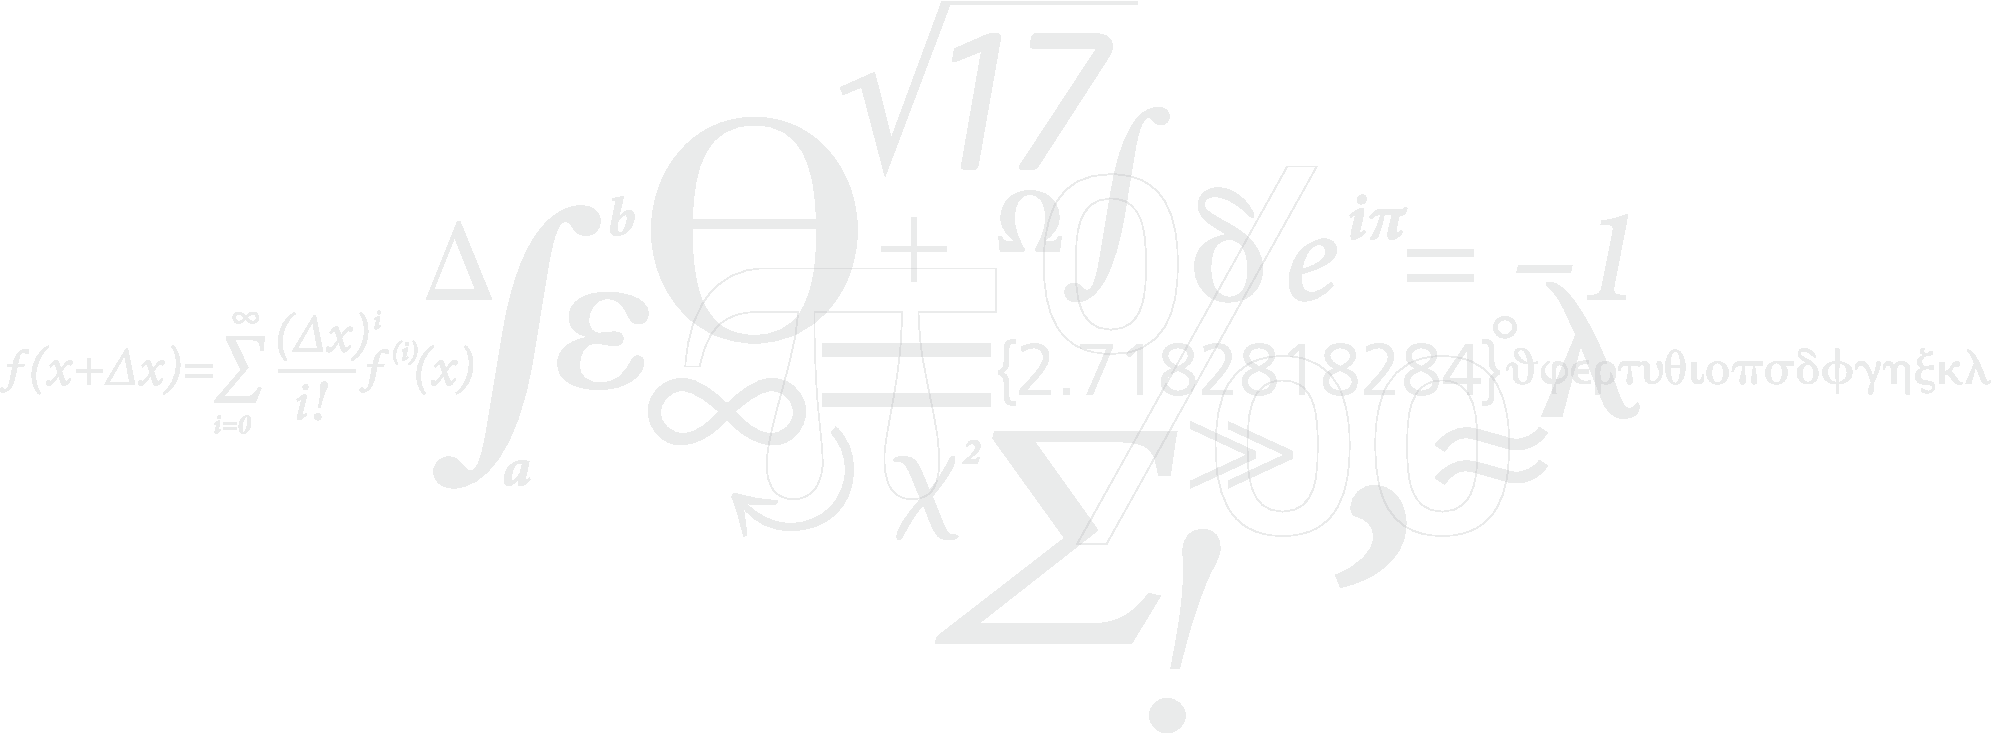
\includegraphics[trim=130mm 0 0 0,width=0.9\textwidth]{DTU-frise-SH-15}
                \vspace*{2.5cm}
            }
        }
    }
}

%!TEX root = ../Thesis.tex

% Text fonts (http://www.macfreek.nl/memory/Fonts_in_LaTeX)
% Install fonts from /usr/local/texlive/<version>/texmf-dist/fonts/opentype/public
\usepackage{fontspec}

% Sans-serif font
\setsansfont[
    Ligatures=TeX,
    Extension=.otf,
    UprightFont=*-regular,
    BoldFont=*-bold,
    ItalicFont=*-italic,
    BoldItalicFont=*-bolditalic,
    %SlantedFont=,
    %BoldSlantedFont=,
    %SmallCapsFont=
]{texgyreadventor}
%\setsansfont[Ligatures=TeX]{Neo Sans Intel}    % Neo Sans Intel – Like DTU font but more symbols
%\setsansfont[Ligatures=TeX]{NeoSans}           % NeoSans – DTU font (missing `+' symbols and other)
%\setsansfont[Ligatures=TeX]{CMU Sans Serif}    % Computer Modern Unicode font
%\setsansfont[Ligatures=TeX]{Latin Modern Sans} % Latin Modern Sans serif font


%!TEX root = ../Thesis.tex

\usepackage{mathtools}    % Det meste matematik (indeholder ams­math og rettelser)
\usepackage{amssymb}
\usepackage{bm}           % Bold symbols
\usepackage{xfrac}        % Flere fracs (\sfrac{}{})
\usepackage{listings}     % Indsæt code
\usepackage{todonotes}    % Cool to-do notes, [disable] skjuler to-dos
\usepackage[backend=biber,bibstyle=ieee,citestyle=numeric-comp]{biblatex} % Benyt BibLaTeX til formatering
\usepackage{subcaption}   % Tillader subfigure, subtable samt \captions
\usepackage{csquotes}
\usepackage{afterpage}
\usepackage{placeins}

%listing settings, æøå support, font config, line number, left lines
\lstset{
    breakatwhitespace=false, breaklines=true,
    inputencoding=utf8, extendedchars=true,
    literate={å}{{\aa}}1 {æ}{{\ae}}1 {ø}{{\o}}1 {Å}{{\AA}}1 {Æ}{{\AE}}1 {Ø}{{\O}}1,
    keepspaces=true, showstringspaces=false, basicstyle=\small\ttfamily,
    frame=L, numbers=left, numberstyle=\scriptsize\color{gray},
    keywordstyle=\color{SteelBlue}\ttfamily,
    stringstyle=\color{IndianRed}\ttfamily,
    commentstyle=\color{Teal}\ttfamily,
} 

\DeclareGraphicsExtensions{.pdf,.eps,.png,.jpg,.gif}	% ændre til .png, .jpg for hurtig visning

\newcommand\defeq{\mathrel{\overset{\makebox[0pt]{\mbox{\tiny def}}}{=}}}


\addbibresource{bibliography/bibliography.bib}

\begin{document}

\pagenumbering{alph}
%!TEX root = ../Thesis.tex 
\thispagestyle{empty}             % No page numbers
\calccentering{\unitlength}
\begin{adjustwidth*}{\unitlength}{-\unitlength}
    \begin{adjustwidth}{-0.5cm}{-0.5cm}
        \sffamily
        \begin{flushright}
            \thesistypeabbr{} Thesis\\*[0cm]
            \thesistype{}\\
        \end{flushright}
        \vspace*{\fill}
        \noindent
        
\includegraphics[width=0.75\textwidth]{DTU-Compute-B-UK}\\*[0.5cm]
        \resizebox{1.08\textwidth}{!}{%
          \Huge \thesistitle{}
        }\\*[0.2cm]
        \LARGE \thesissubtitle{}\\*[1.2cm]
        \parbox[b]{0.5\linewidth}{%
            \large 
            \thesisauthor{}\\*[1.2cm]
            \normalsize
            \thesislocation{} \the\year
        }
        \hfill
\includegraphics[scale=0.7]{DTU-logo-CMYK}
    \end{adjustwidth}
\end{adjustwidth*}
\normalfont
\normalsize

\cleartoevenpage
%!TEX root = ../Thesis.tex
\thispagestyle{empty} % No page numbers
\frieze
\vspace*{\fill}
\noindent
\sffamily
\scriptsize
\textbf{DTU Compute}\\
\textbf{Department of Applied Mathematics and Computer Science}\\
\textbf{Technical University of Denmark}\\
\\
Matematiktorvet\\
Bygning 324\\
2800 Kongens Lyngby, Denmark\\
Phone +45 4525 3031\\
compute@compute.dtu.dk\\
compute.dtu.dk\\
\normalsize
\normalfont
\vspace*{2.5cm}

\clearforchapter

\frontmatter
\pagestyle{plain}
%!TEX root = ../Thesis.tex
\chapter{Summary (English)}

This thesis investigates models for translating between natural languages. The models are based on a recently published model called ByteNet. The ByteNet model is a new approach to neural machine translation that isn't based on attention but instead layers of hierarchical dilated convolutions. Using this approach the ByteNet model runs in linear time while still being resolution persistent.

Using a variation of the ByteNet model, the model is then applied in a semi-supervised settings, where it is trained on both a bilingual and a monolingural dataset. The idea is that the best performing models are typically those that uses the most data. For language pairs where the bilingual dataset is small, monolingural data could be a vital supplement.

Results showed that ByteNet is able to learn natural language translation between from German to English using a bilingual dataset. The model was unfortunately too time consuming to use in a semi-supervised setting for natural language translation. However, a reduced ByteNet model was used to learn a synthetic problem that mimics natural language translation. The semi-supervised experiments showed that monolingural data improves the predictive performance.

\cleardoublepage
%!TEX root = ../Thesis.tex
\chapter{Summary (Danish)}

\cleardoublepage
%!TEX root = ../Thesis.tex
\chapter{Preface}
This thesis was prepared at Department of Applied Mathematics and Computer Science (DTU Compute) at the Technical University of Denmark in fulfillment of the requirements for acquiring an MSc degree in Mathematics. The work was carried out in the period from January 2017 to June 2017.

\vfill

{
\centering
    \thesislocation{} – \thesisdeadline{}\\[1cm]
    \hspace{3cm}
\includegraphics[width=8cm]{Signature.pdf}\\[1cm]
\begin{flushright}
    \thesisauthor{}
\end{flushright}
}

\cleardoublepage
%!TEX root = ../Thesis.tex
\chapter{Acknowledgements}
First and foremost I would like to thank my supervisor Ole Winther for his guidance and support. I would also like to thank Namju Kim, who wrote a quadratic-time implementation of the ByteNet model, which I took much inspiration from. Finally, I would like to thank the DTU HPC team for their fast support.
\tableofcontents
\let\cleardoublepage\clearpage % New chapers starts on next page
\cleartoleftpage
\pagestyle{companion}

\mainmatter
%!TEX root = ../Thesis.tex
\chapter{Introduction}

In the European Parliament, there are 23 officially spoken languages and precise translation is essential for clear communication. Each elected member is not expected to understand all 23 languages, and there isn't a common language that everyone speaks equally well, thus the European Parliament employs translators for translating between these languages \cite{europarl-translation}.

For the European Parliament it is possible to employ translation specialists, and in cases where there aren't someone to translate directly English, French and German are used as relay languages \cite{europarl-translation}. However, translation specialists are not often available to the public.

In India, more than 400 million have internet access, and most of India’s online content is written in English. However, only 20\% of the Indian population speaks English. Excluding English, the nine most used languages in India are: Hindi, Bengali, Marathi, Gujarati, Punjabi, Tamil, Telugu, Malayalam and Kannada. For translating between these languages and English Google have recently started to use Neural Machine Translation in their Google Translate service \cite{google-translate-india}.

Google Translate translates more than 100 billion words each day, for its 500 million users \cite{google-translate-stats}. In the European Parliament, and the United Nations, automatic translation software is also used for assisting the specialists \cite{europarl-translation}. These tools are using for the majority of languages, a technology called ``Statistical machine translation''.

Statistical machine translation (SMT) combines a probability model for the target language, as well as a probability model for mapping between the source and target language. Such a probability model can be a Hidden Markov Model and they will be fitted using a bilingual dataset \cite{smt-comparetive-study}. Bilingual means the dataset contains both the source and target language for each sentence. Previously these models have been word-based, allowing very limited context understand. Recently phrase-based machine translation (PBMT) have been introduced, this allows for much better translation of idioms or multi-word expressions than what has previously been possible. Phrase-based translation is currently the primary strategy used in machine translation. However, even phrase-based translation has a limited understanding of context and can't consider an entire sentence.

Recently advances have been made in applying neural networks to machine translation, this strategy is called neural machine translation (NMT) and has been shown to outperform the current PBMT approaches \cite{google-translate-gnmt}. This approach is able to consider an entire sentence or more and is thus able to understand the context of each word on a level that has not been previously possible.

Beyond being able to process entire sentences, neural machine translation is a more flexible approach than PBMT. As such the NMT strategy is highly relevant for language pairs that have previously been notoriously difficult, such as Chinese to English translation. In September 2016, Google announced that they now used neural machine translation for Chinese to English translation, they are calling this architecture GNMT.

Over the last year, GNMT has been enabled for English, French, German, Spanish, Portuguese, Chinese, Japanese, Korean, Turkish, Russian, Hindi, Vietnamese, Hebrew, and Arabic along with the Indian dialects. These languages are chosen either because there is a huge dataset or because they are notoriously difficult to translate using the existing PBMT strategy. In NMT the quality of the translation is often more dependent on how much data is used, than how advanced the neural architecture is.

In this thesis, NMT will be used to provide German to English translation, and additional effort will be given to applying NMT to ``small'' bilingual dataset. The strategy for applying NMT to ``small'' datasets, is based on the fact that humans, especially babies, are capable of learning languages without prior knowledge. It should thus be possible to use additional non-translated data (monolingual) to train the NMT model. A now almost classical example of using monolingual data to build a language model is the Word2Vec model, this uses the Wikipedia corpus for a single language to create word embeddings. These word embeddings have shown meaningful properties like synonyms being close to each other and relations like $king - man + woman \approx queen$ \cite{word2vec}.

The approach used in this thesis is based on the intuition that translating from for example German to English and then back to German again, should result in the same sentence. This approach does not require the correct English sentence to be known for all sentences, thus a monolingual German dataset can be used. The approach has been shown to yield some improvements \cite{semi-supervised}. This must of cause be used in combination with a bilingual dataset, otherwise the neural network will just learn the identity function. This combination of monolingual and bilingual data is called semi-supervised learning.

There are other approaches for semi-supervised learning, in particular, generative adversarial networks (GAN) has shown good results in computer vision. However, for natural language processing such as NMT, it still lags far behind likelihood based methods \cite{gan-on-nlp}.

The semi-supervised approach does on a theoretical level not depend on the neural translation model. A popular translation model is the Bahdanau Attention model that has shown state-of-the-art performance in machine translation \cite{bahdanau-2015-nmt}. However, the Bahdanau Attention model is a word-based model and for some languages, like German that likes to combine words, it can be advantageous to use characters instead of words as input to the model. While word-based models are currently superior, using characters instead of words eliminates the out-of-dictionary problem that often exists in word-based models.

The out-of-dictionary problem happens because a neural network can only supports a fixed number of outputs, one must thus decide on a fixed dictionary before training the model. Typically 80000 words are used as the dictionary size, if the dictionary becomes much larger than this, it will not be computationally feasible to train the model. 80000 words are not enough to contain every street name and rarely used words, an obvious solution is thus to use characters instead of words. A typical language will not use more than 300 different characters.

While it is possible to use the Bahdanau Attention model with characters as input, the sequences become much longer and this creates certain computational problems. Recently a different approach called ByteNet has been created, this model is specifically character-based and solves the computational problems \cite{bytenet}. The ByteNet model promises high computational performance and achieves state-of-the-art performance compared to other character-based models. Using a computational pragmatic model like ByteNet is essential when one does not have Google-level resources.

The ByteNet model and the semi-supervised approach have never been combined before. In particular, the original paper implementing the semi-supervised approach used the word-based Bahdanau Attention model, which is a drastically different than the ByteNet model.

% Importance of translation
% 1. European parlement % http://www.europarl.europa.eu/multilingualism/trade_of_translator_en.htm 
% 2. Not everybody has human translator, not feasiable to learn it all.
% 3. Indian as an example %https://blog.google/products/translate/making-internet-more-inclusive-india/
% 3b. Statistics for google translate % https://blog.google/products/translate/ten-years-of-google-translate/

% History (SMT) and recent efforts (NMT).
% 4. SMT or PBMT is the current approach.  % https://en.wikipedia.org/wiki/Statistical_machine_translation, % http://acl-arc.comp.nus.edu.sg/archives/acl-arc-090501d3/data/pdf/anthology-PDF/J/J03/J03-1002.pdf
% 5. Issues: Whereas Phrase-Based Machine Translation (PBMT) breaks an input sentence into words and phrases to be translated largely independently, Neural Machine Translation (NMT) considers the entire input sentence as a unit for translation. %  https://research.googleblog.com/2016/09/a-neural-network-for-machine.html
% 6. Google Neural Machine Translation % https://en.wikipedia.org/wiki/Google_Neural_Machine_Translation


% Challenges for language pairs with little interaction.
% 7. most data wins
% 8. language pairs with little data is problematic
% 9. Idea, it is possible to learn a language without foreknowledge, Word2Vec % https://arxiv.org/pdf/1309.4168.pdf
% 10. Learn language separately and use bilingural to learn translation.

% Translation is a difficult problem, be pragmatic.
% 11. GAN is stil very difficult on text (https://arxiv.org/abs/1705.10929).
% 12. Be pragmatic, don't have google level resources.
% 13. ByteNet provides linear-time learning.
% 14. Character-based NMT advantages.
% 15. Semi-Supervised NMT is also very pragmatic.
% 16. ByteNet and Semi-Supervised NMT has never been combined before.

% Extra:
% http://www.cbc.ca/news/canada/british-columbia/tomatoes-google-kelowna-curtis-stone-1.3532564

%!TEX root = ../Thesis.tex
\chapter{Theory}

%!TEX root = ../Thesis.tex
\section{Feed forward Neural Network}
\label{sec:theory:ffnn}

Neural Machine Translation is based on the neural network framework. Modern networks are extreamly complex and uses rather advanced operations such as convolution, others uses complex combinations of simpler operations such as the LSTM block. To give a short introduction to this framework the feed forward neural network (FFNN) is presented. This is the simplest type in the neural network familiy. As such it doesn't have much use for translation, but the more advanced neural networks can be seen as extensions of a feed forward neural network.

\subsection{The neuron}

The neuron is the main component in any neural network. Mathematically it is just a function which takes a vector and returns a scalar. It does this by a weighted sum of the inputs $\{ x_i \}_{i=1}^I$ and by adding a bias value $b$. The sum is then then typically transformed using a non-linear function $\theta$.
\begin{equation}
a = \theta(z),\quad z = \sum_{i=1}^I w_{i} x_i + b
\end{equation}

The value $a$ is the output of the neuron and is called the \textit{activation}. In the past the sigmoid function $\sigma(\cdot)$ and the hyperbolic tangent $\tanh(\cdot)$ function have been very popular\cite{bishop}, but recently the rectified linear unit (ReLU) $\theta(z) = \max(0, z)$ has become the norm. If no non-linear function is applied then the identity function $\theta(a) = a$ is used.

\begin{figure}[H]
	\centering
	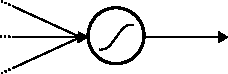
\includegraphics[scale=1]{theory/ffnn-neuron}
	\caption{Visual representation of a single neuron. The left arrows represents the input elements $\{ x_i \}_{i=1}^I$. The circle represent the function that returns the activation scalar $a$ (right arrow).}
\end{figure}

\subsection{The network}

A feed forward neural network is in its simplest form a \textit{multivariate non-linear regression model} constructed by combining neurons. Such a regression model can then be turned into a classification model by adding a softmax transformation \cite{the-elements-of-statistical-learning} to the output. By doing this each output value becomes the class probability $y_k = P(C_k | x)$.

\begin{figure}[h]
	\centering
	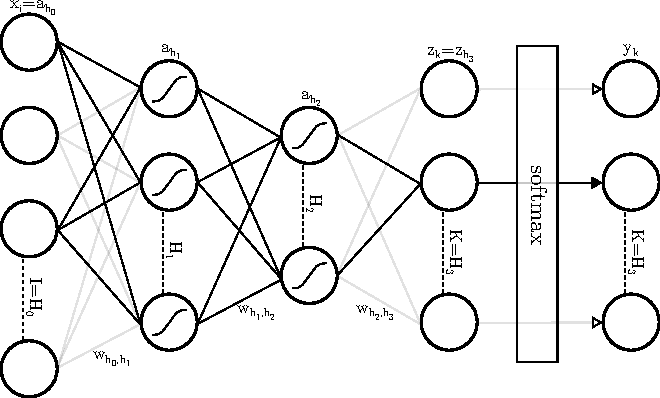
\includegraphics[scale=1]{theory/ffnn-network.pdf}
	\caption{Visual representation of a neural network with two hidden layers. Some lines are less visible, this is just a visual aid because the many connections can be difficult to look at.}
	\label{fig:theory:ffnn:network}
\end{figure}

The neural network in Figure \ref{fig:theory:ffnn:network}, have one input layer $x_i, i \in [1, I]$ and one output layer $y_k, k \in [1, K]$. This is the same for any neural network, what varies is the type of network (here a feed forward neural network) and the amount of hidden layers (here two). The hidden layers are typically the layers that contains the non-linear transformation functions. If there are no hidden layers, the neural network is just a multiclass logistic regressor\cite{bishop}.

Because there are more than one neuron in each layer and many layers, the neuron index and layer index is denoted by the subscript. For example a neuron output is denoted by $a_{h_{\ell}}$ for $h_{\ell} \in [1, H_{\ell}]$, where $h_{\ell}$ is the neuron index and $H_\ell$ is the amount of neurons in layer $\ell$.

\subsection{Forward pass}

Calculation of the network output ($y_k$) is sometimes called the \textit{forward pass}, while the parameter estimation is sometimes called the \textit{backward pass}.

The \textit{forward pass} is simply calculated by applying the neuron function to all nerons in all layers. By defining $a_{h_0} = x_i$ the \textit{forward pass} can be generalized to any amount of hidden layers ($L$):
\begin{equation}
\begin{aligned}
a_{h_\ell} &= \theta(z_{h_\ell}), && \forall h_{\ell} \in [1, H_{\ell}], \ell \in [1, L] \\
z_{h_\ell} &= \sum_{h_{\ell-1} = 1}^{H_{\ell-1}} w_{h_{\ell-1}, h_{\ell}} a_{h_{\ell-1}} + b_{h_{\ell}}, && \forall \ell \in [1, L+1] \text{ where: } a_{h_0} = x_i, H_0 = I \\
\end{aligned}
\end{equation}

Note that the last layer $\ell = L + 1$ does not use the non-linear transformation function $\theta$, instead it uses the softmax function.
\begin{equation}
\begin{aligned}
y_k = \frac{\exp(z_k)}{\sum_{k'=1}^K \exp(z_{k'})}, && \forall k \in [1, K] \text{ where: } z_k=z_{h_{L+1}}, K = H_{L + 1}
\end{aligned}
\label{eq:theory:ffnn:y}
\end{equation}

The $z_k$ values there are feed to the softmax function are often called \textit{logits}, because they are unnormalized log properbilities ($\exp(z_k) \propto y_k$). This has some advantages, for example if one wants the most likely label given $\mathbf{x}$ one can just find the largest $z_k$ and thus skip the softmax, which can otherwise be quite expensive to calculate.

\subsection{Loss function}

Optimization of the parameters $w_{i,j}$ and $b_{j}$ requires definition of a loss function. For classification it makes sense to maximize the joint probability of observing all the observations:
\begin{equation}
P(\mathbf{t} | \mathbf{x}, \mathbf{w}, \mathbf{b}) = \prod_{n=1}^N P(\mathbf{t}_n | \mathbf{x}_n, \mathbf{w}, \mathbf{b})  = \prod_{n=1}^N \prod_{k=1}^K P(C_{n, k} | \mathbf{x}_n, \mathbf{w}, \mathbf{b})^{t_{n, k}}
\end{equation}

Here $\mathbf{x}_{n}$ is the input vector for observation $n$, with a corresponding label vector $\mathbf{t}_n$. The label vector is an indicator vector constructed using 1-of-K encoding. The class probability $P(C_{n, k} | \mathbf{x}_n, \mathbf{w}, \mathbf{b})$ is $y_k$ from the \textit{forward pass} for observation $n$.

The logarithm is then used to create linearity and avoid numerical floating point issues. The sign is also changed such that it becomes a loss function:
\begin{equation}
- \ln\left(P(\mathbf{t} | \mathbf{x}, \mathbf{w}, \mathbf{b})\right) = - \sum_{n=1}^N \sum_{k=1}^K t_{n, k} \ln\left( P(C_{n, k} | \mathbf{x}_n, \mathbf{w}, \mathbf{b})\right)
\label{eq:theory:ffnn:long-loss}
\end{equation}

Because of the linearity in \eqref{eq:theory:ffnn:long-loss} it makes sense to just consider the loss function for one datapoint, thus the $n$ index can be omitted. This gives the final loss function which is denoted by $\mathcal{L}$:
\begin{equation}
\mathcal{L} = - \sum_{k=1}^K t_{k} \ln\left( P(C_{k} | \mathbf{x}, \mathbf{w})\right) =  - \sum_{k=1}^K t_k \ln(y_k)
\label{eq:theory:ffnn:loss}
\end{equation}

The formulation \eqref{eq:theory:ffnn:loss} is particularly useful as it allows for some numerical stability tricks, see Appendix \ref{appendix:numerical-stability:cross-entropy} \todo{\url{https://github.com/tensorflow/tensorflow/blob/master/tensorflow/core/kernels/sparse_xent_op.h\#L190L219}}.

\subsection{Backward pass}

For the neural network there is no closed form solution to optimizing the loss function. Instead gradient based optimization algorithms are used. Gradient based optimization uses the derivatives of the loss function with respect to the parameters to iteratively optimize the parameters. This approach will be discussed in Section \ref{sec:theory:optimization}, for now the important part is calculate the derivatives:
\begin{equation}
\begin{aligned}
\frac{\partial \mathcal{L}}{\partial w_{h_{\ell-1}, h_\ell}} \wedge \frac{\partial \mathcal{L}}{\partial b_{h_\ell}}, && \forall \ell \in [1, L + 1]
\end{aligned}
\label{eq:theory:ffnn:bprop-problem}
\end{equation}

For calculating the derivatives the \textit{error backpropagation} algorithm is used, this algorithm results in what is called the \textit{backward pass}.

The main trick in \textit{error backpropagation} is to define the partial derivative $\delta_{h_\ell}$, this is then used for bookkeeping and is what makes it feasiable to calculate the derivatives.
\begin{equation}
\delta_{h_\ell} \defeq \frac{\partial \mathcal{L}}{\partial z_{h_\ell}}
\end{equation}

Using this defintion the chain rule can be applied on \eqref{eq:theory:ffnn:bprop-problem}:
\begin{equation}
\begin{align}
\frac{\partial \mathcal{L}}{\partial w_{h_{\ell-1}, h_\ell}} &= \frac{\partial \mathcal{L}}{\partial z_{h_\ell}} \frac{\partial z_{h_\ell}}{\partial w_{h_{\ell-1}, h_\ell}} &&= \delta_{h_\ell} a_{h_{\ell-1}},&& \forall \ell \in [1, L+1],\quad a_{h_0} = x_i \\
\frac{\partial \mathcal{L}}{\partial b_{h_\ell}} &= \frac{\partial \mathcal{L}}{\partial z_{h_\ell}} \frac{\partial z_{h_\ell}}{\partial b_{h_\ell}} &&= \delta_{h_\ell},&& \forall \ell \in [1, L+1]
\end{align}
\end{equation}


Calculating $\delta_{h_\ell}$ is a bit more involved since $z_{h_\ell}$ affects more than one intermediate variable, but even so the chain rule can still be applied:
\begin{equation}
\begin{aligned}
\delta_{h_\ell} = \frac{\partial \mathcal{L}}{\partial z_{h_\ell}} &= \frac{\partial \mathcal{L}}{\partial a_{h_\ell}} \frac{\partial a_{h_\ell}}{\partial z_{h_\ell}} \\
&= \theta'(z_\ell) \sum_{h_{\ell+1}}^{H_{\ell+1}} \frac{\partial \mathcal{L}}{\partial z_{\ell+1}} \frac{\partial z_{\ell+1}}{\partial a_\ell} \\
&= \theta'(z_\ell) \sum_{h_{\ell+1}}^{H_{\ell+1}} \delta_{h_{\ell+1}} w_{h_\ell, h_{\ell+1}}, \forall \ell \in [1, L]
\end{aligned}
\label{eq:theory:ffnn:bprop}
\end{equation}

The last delta $\delta_{h_{L+1}}$ is diffrent but can still be calculated by using the chain rule.
\begin{equation}
\delta_{h_{L + 1}} = \delta_k = \frac{\partial \mathcal{L}}{\partial z_k} = \sum_{k'=1}^K \frac{\partial \mathcal{L}}{\partial y_{k'}} \frac{\partial y_{k'}}{\partial z_k}
\label{eq:theory:ffnn:bprop-deltaK}
\end{equation}

The first derivative $\frac{\partial \mathcal{L}}{\partial y_{k'}}$ can be derived from \eqref{eq:theory:ffnn:loss}:
\begin{equation}
\frac{\partial \mathcal{L}}{\partial y_{k'}} = \frac{\partial}{\partial y_{k'}} \left(- \sum_{k''=1}^K t_{k''} \ln(y_{k''})\right) = -\frac{t_{k'}}{y_{k'}}
\label{eq:theory:ffnn:bprop-Ldy}
\end{equation}

The other derivative $\frac{\partial y_{k'}}{\partial z_k}$ can be derived from \eqref{eq:theory:ffnn:y}:
\begin{equation}
\begin{aligned}
\frac{\partial y_{k'}}{\partial z_k}
&= \frac{\partial}{\partial z_k} \frac{\exp(z_{k'})}{\sum_{k''=1}^K \exp(z_{k''})} \\
&= \frac{\frac{\partial}{\partial z_k} \exp(z_{k'})}{\sum_{k''=1}^K \exp(z_{k''})}
- \frac{\exp(z_{k'}) \frac{\partial}{\partial z_k} \sum_{k''=1}^K \exp(z_{k''})}{\left(\sum_{k''=1}^K \exp(z_{k''})\right)^2} \\
&= \frac{\frac{\partial}{\partial z_k} \exp(z_{k'})}{\sum_{k''=1}^K \exp(z_{k''})}
- \frac{\exp(z_{k'})}{\sum_{k''=1}^K \exp(z_{k''})} \frac{\frac{\partial}{\partial z_k} \sum_{k''=1}^K \exp(z_{k''})}{\sum_{k''=1}^K \exp(z_{k''})}
\end{aligned}
\end{equation}

Because of the difference in index, the first term is only not zero when $k = k'$, in which case $y_k$ is the derivative. It thus becomes useful to define:
\begin{equation}
\delta_{i,j} = \begin{cases}1& \text{when } i = j \\ 0 & \text{otherwise}\end{cases}
\end{equation}

Similarly in the second term $\frac{\partial}{\partial z_k} \exp(z_{k''})$ is zero except in the case where $k = k''$:
\begin{equation}
\frac{\partial y_{k'}}{\partial a_k} = \delta_{k, k'} y_k - y_{k'} y_k
\label{eq:theory:ffnn:bprop-yda}
\end{equation}

The result from \eqref{eq:theory:ffnn:bprop-Ldy} and \eqref{eq:theory:ffnn:bprop-yda} is then combined into \eqref{eq:theory:ffnn:bprop-deltaK}:
\begin{equation}
\begin{aligned}
\delta_{h_{L + 1}} = \delta_k &= \sum_{k'=1}^K -\frac{t_{k'}}{y_{k'}} \left( \delta_{k, k'} y_k - y_{k'} y_k \right) = \sum_{k'=1}^K -\frac{t_{k'}}{y_{k'}} \delta_{k, k'} y_k + \sum_{k'=1}^K \frac{t_{k'}}{y_{k'}} y_{k'} y_k \\
&= -\frac{t_k}{y_k} y_k + y_k \sum_{k'=1}^K t_{k'} = -t_k + y_k = y_k - t_k
\end{aligned}
\label{eq:theory:ffnn:bprop-deltaKfinal}
\end{equation}

To get $\sum_{k'=1}^K t_{k'} = 1$ it's used that $\{ t_{k'} \}_{k'=1}^K$ is the target distribution and thus must sum to 1.

Using \eqref{eq:theory:ffnn:bprop-deltaKfinal} and \eqref{eq:theory:ffnn:bprop} all $\delta_{h_\ell}$ for $\ell \in [1, L+1]$ can be calculated for a feed forward neural network with $L$ hidden layers. Note how \eqref{eq:theory:ffnn:bprop-deltaKfinal} is an error measure and this value is propagated back through the network by the $\delta_{h_\ell}$ equations in \eqref{eq:theory:ffnn:bprop}. This is why the method is called \textit{error backpropagation}.

\clearpage

\section{Gradient Based Optimization}
\subsection{Gradient Desent Optimization}
\subsection{Adam Optimization}
\clearpage

\section{Convolution Neural Network}
\subsection{Diliated Convolution}
\subsection{Forward Pass}
\subsection{Backward Pass}
\clearpage

\section{Improving Convergence Speed}
\label{sec:convergence}

A good optimization algorithm is essential for fitting a deep neural network, however the convergence rate can often be improved by modifying the network architecture itself such that the cost function is easier to optimize. These modifications do not radically alter the network, but rather modifies existing layers. The modifications can become the identity function through parameter optimization and thus doesn't change the theoretical capabilities of the neural network.

\subsection{Batch Normalization}
Traditionally in feed forward neural networks, it has been the norm to standardize the input to have zero mean and unit variance.
\begin{equation}
\hat{x}_i = \frac{x_i - \mathbb{E}[x_i]}{\sqrt{\textsc{Var}[x_i] + \epsilon}}, \quad \forall i \in [1, I]
\end{equation}

This standardization places the input to the sigmoid activation function in its linear domain ($\sigma(\epsilon) \approx \epsilon, \forall \epsilon \in [-1, 1]$), which is a reasonable starting point for the optimization \todo{[LeCun et al., 1998b; Wiesler \& Ney, 2011]}. Batch normalization extends this idea to standardize before all activation functions in a deep neural network. This has positive consequences beyond limiting the sigmoid activation to its linear domain \cite{batch-normalization}.

Consider a neural network with just one hidden layer:
\begin{equation}
\mathcal{L}(\mathbf{t}, \mathbf{W}_2 \theta(\mathbf{W}_1 \mathbf{x} + \mathbf{b}_1) + \mathbf{b}_2)
\end{equation}
When optimizing the loss function, the parameters $\mathbf{W}_1, \mathbf{W}_2, \mathbf{b}_1$ and $\mathbf{b}_2$ are all optimized simultaneously. Furthermore, the optimization of $\mathbf{W}_2, \mathbf{b}_2$ does directly depend on $\theta(\mathbf{W}_1 \mathbf{x} + \mathbf{b}_1)$ though the error term. This becomes an issue when the distribution of $\theta(\mathbf{W}_1 \mathbf{x} + \mathbf{b}_1)$ changes because the updated $\mathbf{W}_2$ and $\mathbf{b}_2$ assumes the original distribution. This change of the distribution of the internal activations is called an \textit{internal covariate shift}. \cite{batch-normalization}.

The \textit{internal covariate shift} issue can be illustrated by considering a scalar $a = w x + b \sim \mathcal{N}(b, w)$, as it would appear in a very simple neural network, the sigmoid activation function is then applied on $\mathcal{N}(b, w)$ by using the \textit{change of variable theorem}. Using this one can change $w$ and $b$ and observe how the sigmoid activation distribution changes (Figure \ref{fig:convergence:batch-norm:activation-distribution}).

\begin{figure}[h]
	\centering
	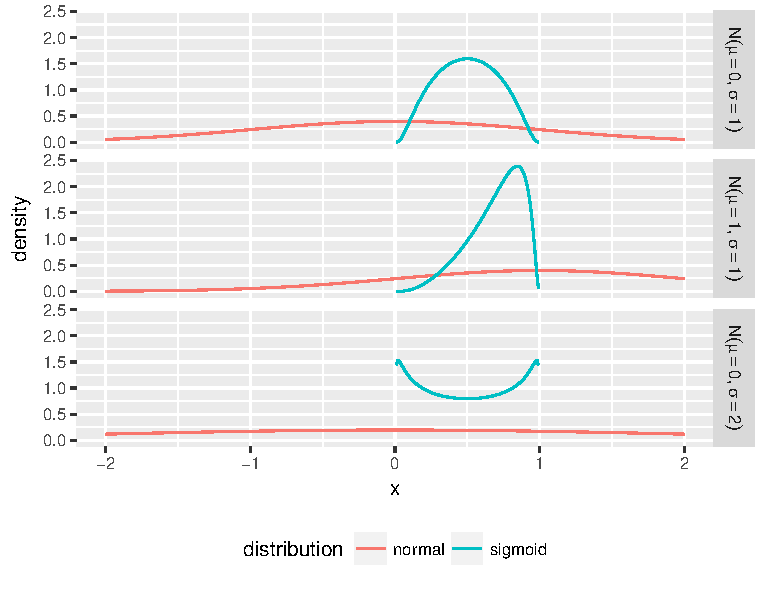
\includegraphics[scale=1]{theory/batch-norm-activation-distribution}
	\caption{Shows $X \sim \mathcal{N}(\mu, \sigma)$ and $\mathrm{sigmoid}(X)$ calculated using the \textit{change of variable theorem}.}
	\label{fig:convergence:batch-norm:activation-distribution}
\end{figure}

\subsubsection{A solution}
The \textit{internal covariate shift} issue can in practice be solved by using a small learning rate. However, this is not an optimal solution as it prolongs the optimization. Batch normalization is an alternative solution, that solves the issue by standardizing the input to the activation function. To truly standardize this input the covariance matrix, as well as its inverse square root, should be calculated. These calculations are very expensive, thus batch normalization makes a practical compromise by only standardizing using the variance.
\begin{equation}
\hat{z}_{h_\ell} = \frac{z_{h_\ell} - \mathbb{E}[z_{h_\ell}]}{\sqrt{\textsc{Var}[z_{h_\ell}] + \epsilon}}, a_{h_\ell} = \theta(\hat{z}_{h_\ell})
\end{equation}

The expectation ($\mathbb{E}[z_{h_\ell}]$) and variance ($\textsc{Var}[z_{h_\ell}]$) themselves are expensive to estimate over the entire dataset, thus it's only done over each mini-batch. This also makes it much more feasible to integrate the standardization into the backward pass. Note also that because the expectation is subtracted, the bias $b_{h_\ell}$ in $z_{h_\ell}$ has no effect and should thus be omitted:
\begin{equation}
z_{h_\ell} = \sum_{h_{\ell-1}}^{H_{\ell-1}} w_{h_{\ell-1}, h_\ell} a_{h_{\ell-1}} 
\end{equation}


Finally, to allow batch normalization to become the identity function, two more parameters ($\gamma, \beta$) are added to the optimization problem:
\begin{equation}
\hat{z}_{h_\ell} = \gamma_{h_\ell} \frac{z_{h_\ell} - \mathbb{E}[z_{h_\ell}]}{\sqrt{\textsc{Var}[z_{h_\ell}] + \epsilon}} + \beta_{h_\ell}, a_{h_\ell} = \theta(\hat{z}_{h_\ell})
\label{eq:theory:convergence:batch-norm}
\end{equation}

The backward pass for learning ($w, \gamma, \beta$) is rather complicated, but computationally completely feasible as long as the mini-batch size is small. See Appendix \ref{appendix:backward-pass:batch-norm} for the backward pass.

In the special case that $\theta(\cdot)$ is multiplicative linear with respect to a scalar (i.e. $\theta(\alpha \hat{z}_{h_\ell}) = \alpha \theta(\hat{z}_{h_\ell})$) and the following layer isn't sensitive to a multiplication factor, then $\gamma_{h_\ell}$ can be removed from the optimization. A common case is where $\theta(\cdot)$ is the ReLU function, in this case:
\begin{equation}
\begin{aligned}
\alpha_{h_\ell} = \mathrm{ReLU}(\hat{z}_{h_\ell}) &= \gamma_{h_\ell} \mathrm{ReLU}\left(\frac{z_{h_\ell} - \mathbb{E}[z_{h_\ell}]}{\sqrt{\textsc{Var}[z_{h_\ell}] + \epsilon}} +  \frac{1}{\gamma_{h_\ell}}\beta_{h_\ell}\right)\\
&= \gamma_{h_\ell} \mathrm{ReLU}\left(\frac{z_{h_\ell} - \mathbb{E}[z_{h_\ell}]}{\sqrt{\textsc{Var}[z_{h_\ell}] + \epsilon}} +  \tilde{\beta}_{h_\ell}\right)
\end{aligned}
\end{equation}

In the next layer $\alpha_{h_\ell}$ is then multiplied by some other weight that $\gamma_{h_\ell}$ can be merged into. This simplification can often be applied and can be quite valuable as it removed some computations and further simplifies the loss curvature.

\subsubsection{Inference}

With an established backward pass, the network can easily be trained. However, there is still an open question about how inference should be done.

The inference should be deterministic once training is done, thus the ideal solution would be to use the estimated expectation and variance from the entire training dataset in \eqref{eq:theory:convergence:batch-norm}. However, because this calculation can be rather expensive a more practical solution is to use a moving average. Let's denote $\sigma^2_{\mathcal{B}_i}$ and $\mu_{\mathcal{B}_i}$ as the variance and mean estimate after mini-batch $i$. Then in addition to the optimization of ($w, \gamma, \beta$), $\sigma^2_{\mathcal{B}_i}$ and $\mu_{\mathcal{B}_i}$ will also update during training.
\begin{equation}
\begin{aligned}
\sigma^2_{\mathcal{B}_i} &= \lambda \sigma^2_{\mathcal{B}_{i-1}} + (1 - \lambda) \textsc{Var}[z_{h_\ell}] \\
\mu_{\mathcal{B}_i} &= \lambda \mu_{\mathcal{B}_{i-1}} + (1 - \lambda) \mathbb{E}[z_{h_\ell}]
\end{aligned}
\end{equation}

At inference $\hat{z}_{h_\ell}$ are then calculated using $\sigma^2_{\mathcal{B}_i}$ and $\mu_{\mathcal{B}_i}$.

\begin{equation}
\hat{z}_{h_\ell} = \gamma_{h_\ell} \frac{z_{h_\ell} - \mu_{\mathcal{B}_i}}{\sqrt{\sigma^2_{\mathcal{B}_i} + \epsilon}} + \beta_{h_\ell}, a_{h_\ell} = \theta(\hat{z}_{h_\ell})
\end{equation}

\subsubsection{Weight sharing network}

Because it is the weight changes that causes an \textit{internal covariate shift}, the normalization should happen over all $z_{h_\ell}$ values that use these weights. Thus in RNN, the normalization should also be done over time, and in CNN the normalization should also happen over the ``image''. This works well for actual images, however in RNN and CNN that describes a causal relation, the mean and variance at any time step (e.g. $t=0$) will contain information from all time steps, which breaks the causality of the network. This issue in practice be solved by not normalizing over time, however, if the sequences aren't all of the same lengths then the mean and variance estimation for the last time step will be extremely poor.

\subsection{Layer Normalization}

Layer normalization attempts to solve the issues that exist when batch normalization is applied to causal weight sharing networks. It does this by not normalization over the batch, but normalizing over the $\{z_{h_\ell}\}_{h_\ell=1}^{H_\ell}$ vector. \cite{layer-normalization}

\begin{displayquote}
Notice that changes in the output of one layer will tend to cause highly correlated changes in the summed inputs to the next layer, especially with ReLU units whose outputs can change by a lot. This suggests the “covariate shift” problem can be reduced by fixing the mean and the variance of the summed inputs within each layer. \todo{understand this}
\end{displayquote}

Normalizing over the summed inputs $z_{h_\ell}$ results in the following forward pass:
\begin{equationbox}[H]
Activation:
\begin{equation*}
\begin{aligned}
z_{h_\ell} &= \sum_{h_{\ell-1}}^{H_{\ell-1}} w_{h_{\ell-1},h_\ell} a_{h_\ell-1} \\
\hat{z}_{h_\ell} &= \gamma_{h_\ell} \frac{z_{h_\ell} - \mu_{\ell}}{\sqrt{\sigma_{\ell}^2 + \epsilon}} + \beta_{h_\ell} \\
a_{h_\ell} &= \theta\left(z_{h_\ell}\right)
\end{aligned}
\end{equation*}
Statistics:
\begin{equation*}
\begin{aligned}
\mu_{\ell} &= \frac{1}{H_\ell} \sum_{h_\ell}^{H_\ell} z_{h_\ell} \\
\sigma_{\ell}^2 &= \frac{1}{H_\ell} \sum_{h_\ell}^{H_\ell} (z_{h_\ell} - \mu_{\ell})^2
\end{aligned}
\end{equation*}
\caption{Forward equations for Layer Normalization.}
\end{equationbox}

Note that the bias $b_{h_\ell}$ is excluded here for a different reason than what was the case in batch normalization. In batch normalization $b_{h_\ell}$ was a constant and is thus removed when the mean is subtracted. In layer normalization, the mean is over $h_\ell \in [1, H_\ell]$ and thus $b_{h_\ell}$ is no longer a constant. However the original reasoning for layer normalization ``output of one layer will tend to cause highly correlated changes in the summed inputs'' \cite{layer-normalization}, does not include $b_{h_\ell}$ in ``summed inputs'' and thus the normalization should only happen over $\sum_{h_{\ell-1}}^{H_{\ell-1}} w_{h_{\ell-1},h_\ell} a_{h_\ell-1}$. As such $\hat{z}_{h_\ell}$ actually becomes
\begin{equation*}
\hat{z}_{h_\ell} = \gamma_{h_\ell} \frac{z_{h_\ell} - \mu_{\ell}}{\sqrt{\sigma_{\ell}^2 + \epsilon}} + b_{h_\ell} + \beta_{h_\ell},
\end{equation*}
but $ b_{h_\ell}$ then becomes redundant because of $\beta_{h_\ell}$.

The backward pass for learning ($w, \gamma, \beta$) is like in batch normalization a bit complicated, see Appendix \ref{appendix:backward-pass:batch-norm} for the backward pass.

Similar to batch normalization the $\hat{z}_{h_\ell}$ calculation can be simplified if $\theta(\cdot)$ is multiplicative linear (i.e. $\theta(\alpha \hat{z}_{h_\ell}) = \alpha \theta(\hat{z}_{h_\ell})$) and $\gamma_{h_\ell}$ can be merged into a weight in the following layer.

\subsubsection{Properties}

Batch normalization and layer normalization have somewhat similar properties, as shown in Table \ref{table:convergence:layer-norm:properties}. \textit{Weight matrix re-centering invariance} is likely the most important property, as bad weight matrix initialization is often the cause of slow convergence. 

\begin{table}[H]
\centering
\begin{tabular}{r|p{2cm} p{2cm} p{2cm} p{2cm}}
	           & Weight matrix re-scaling & Weight matrix re-centering & Dataset re-scaling& Dataset re-centering \\ \hline
	Batch norm & Invariant & No & Invariant & Invariant \\
	Layer norm & Invariant & Invariant & Invariant & No \\
\end{tabular}
\caption{Invariance properties when using batch or layer normalization. Also, note that batch normalization is invariant to \textit{Weight vector re-scaling} and layer normalization is invariant to \textit{Single training case re-scaling} \cite{layer-normalization}.}
\label{table:convergence:layer-norm:properties}
\end{table}

Another difference between batch and layer normalization is that in layer normalization it is not necessary to maintain a moving average over $\mu$ and $\sigma^2$ for inference, as these are estimated per observation.

\subsubsection{Experimental Results}

In the original paper \cite{layer-normalization} they showed that layer normalization outperforms batch normalization in RNNs. batch normalization is however the preferred choice in CNN, though layer normalization still performs better than the non-normalized baseline. It is theoretically unclear why layer normalization performs poorly on CNNs, but a possible explanation is that there is an underlying assumption that the hidden units $a_{h_\ell}$ make similar contributions, in CNN the hidden units typically represents very different things (e.g. ear, mouth, hair) thus some will be very inactive while others will be very active.

\subsection{Residual Learning}

The most sophisticated neural networks are typically rather deep networks with many layers, thus it is easy to think that ``deeper is better''. However it turns that this is not necessarily true. First of all, there is a vanishing/exploding gradient problem, but recently with good normalization and weight initialization, this is becoming less significant. It turns out that adding layers to a networks that already works well can degrade performance. This is not just a matter of overfitting as also the training error degrades \cite{residual-learning}.

In theory, if there are too many layers the network should optimize such that some of the layers simply becomes the identity function. However, even modern day optimizers are not able to find such a solution. Residual learning solves this problem, by changing the network architecture such that the optimization problem is easier to solve. If the desired function is denoted $\mathcal{H}(\mathbf{x})$, residual learning solves the issue by changing optimization problem such it should find $\mathcal{F}(\mathbf{x}) \defeq \mathcal{H}(\mathbf{x}) - \mathbf{x}$ instead. This is done by transforming the layer to be $\mathcal{F}(\mathbf{x}) + \mathbf{x}$.

\begin{figure}[H]
    \centering
    \begin{subfigure}[b]{0.4\textwidth}
        \centering
        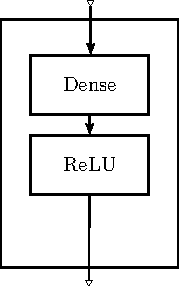
\includegraphics[scale=1]{theory/convergence-nonresidual-layer.pdf}
        \caption{Traditional Dense-ReLU layer}
    \end{subfigure}
    ~ %
    \begin{subfigure}[b]{0.4\textwidth}
        \centering
        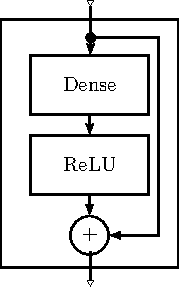
\includegraphics[scale=1]{theory/convergence-residual-layer.pdf}
        \caption{Residual Dense-ReLU layer}
    \end{subfigure}
    \caption{Comparison of traditional and residual Dense-ReLU layer}
\end{figure}

The idea is that getting $\mathcal{F}(\mathbf{x}) = 0$ is a lot easier to solve than $\mathcal{H}(\mathbf{x}) = \mathbf{x}$. For both the ReLU and sigmoid transformation, $\mathcal{F}(\mathbf{x}) = 0$ can be obtained by moving the weights to some extreme, while $\mathcal{H}(\mathbf{x}) = \mathbf{x}$ is drastically more difficult, particularly for the sigmoid case. If the layer really needs a non-trivial $\mathcal{H}(\mathbf{x})$ function, the optimizer simply needs to find $\mathcal{H}(\mathbf{x}) - \mathbf{x}$, which should not be that much more difficult.

A downside of using a residual layer is that the output dimension must match the dimension of $\mathbf{x}$. However there are workarounds, for example, one can add an extra dense layer to change the dimensionality of either the output dimension or $\mathbf{x}$.
\clearpage

\section{ByteNet}
\subsection{ByteNet Residual Block}
\subsection{Encoder}
\subsection{Decoder}
\subsection{Forward Pass}
\clearpage

\section{Semi-Supervised Learning for NMT}
\subsection{Forward Pass}
\subsection{Backward Pass}
\subsection{Monte-Carlo Expectation Estimation}
\clearpage
\cleartorecto
%!TEX root = ../Thesis.tex
\chapter{Results}


\section{Problems and Datasets}

3 Datasets will be used to evaluate the ByteNet and semi-supervised ByteNet models. The WMT Translation Task provides a large corpus of text in form of different datasets. Two datasets are used in this thesis, the Europarl v7 dataset and the WMT NewsTest dataset. For validating the implementation and discussing the model a very simple synthetic dataset is also used, this dataset is named ``Synthetic Digits''.

\subsection{WMT Translation Task}

Each year WMT holds a conference on machine translation, this works as a series of workshops and competitions on different translation tasks. One of these translation tasks are on news translation \cite{wmt16}. The task is to translate paragraphs from news articles to another language. The translations are evaluated on the WMT NewsTest dataset, that are from news articles collected over a specific year. The news translation task is the primary translation task that NMT papers evaluates their models on \cite{bytenet, bahdanau-2015-nmt, sutskever-2014-nmt}.

\begin{table}[H]
\centering
\begin{tabular}{r|p{5cm} p{5cm}}
	obs. & source & target\\ \hline
     0 & Die Premierminister Indiens und Japans trafen sich in Tokio. & India and Japan prime ministers meet in Tokyo \\
     1 & Pläne für eine stärkere kerntechnische Zusammenarbeit stehen ganz oben auf der Tagesordnung. & High on the agenda are plans for greater nuclear co-operation. \\
     2 & Berichten zufolge hofft Indien darüber hinaus auf einen Vertrag zur Verteidigungszusammenarbeit zwischen den beiden Nationen. & India is also reportedly hoping for a deal on defence collaboration between the two nations.
\end{tabular}
\caption{Example form the WMT NewsTest 2015 de-en dataset.}
\end{table}

The WMT NewsTest is about 3000 sentences each year, this is not enough data to build a good translation model. To that end WMT provides additional datasets for training, most importantly is the Europarl v7 dataset. The Europarl dataset contains high quality translations of various of documents from the European Parlement \cite{europarl}. While this dataset is a huge high quality dataset it is also heavily biased, as some word grams like ``The European Parlement'' appears much more often that in the NewsTest dataset.

A few of the sequences in Europarl v7 are rather long (3000+ characters), including these causes out of memory issues on the GPU, thus only sequence pairs where both the source and target sequence is less than 500 are included. This sequence length was chosen because no sequence in the WMT NewsTest is longer than 500 characters. 

\begin{table}[H]
\centering
\begin{tabular}{r|p{5cm} p{5cm}}
	obs. & source & target\\ \hline
        0 & Wir sind nach wie vor der Ansicht, daß der wirtschaftliche und soziale Zusammenhalt ein zentrales Ziel der Union ist. & We still feel that economic and social cohesion is one of the Union' s fundamental objectives. \\
        1 & Den Kommissar möchte ich auffordern, in diesen beiden Bereichen tätig zu werden und uns dabei mit einzubinden. & These are two areas of action which I invite the Commissioner to set up and in which I would ask him to involve us. \\
        2  & Dies zwingt das Europäische Parlament, den Herrn Kommissar und die Kommission zu entschlossenem strategischen Handeln. & This fact means that the European Parliament, the Commissioner and the Commission must act decisively and strategically.
\end{tabular}
\caption{Example form the Europarl v7 de-en dataset.}
\end{table}

\subsection{Synthetic Digits}

While WMT Translation Task is good problem to measure a translation model on, it is a complex problem that takes a long time for a neural network to learn. It is also not obvious if a model will be able to solve this problem at all. In particular the Semi-Supervised ByteNet model has never been attempted before, thus it is meaning full to validate that it can solve a simple problem before attempting more a more complex problem like the WMT Translation Task.

The synthetic digits dataset is simply a uniformly random sequence of integers. In the source each digit is spelled out in english, in the target each digit is represented as a symbol. The sequence length is uniformly randomly chosen to be either 2 or 3 digits long.
\begin{table}[H]
\centering
\begin{tabular}{r|p{5cm} p{5cm}}
	obs. & source & target\\ \hline
	0 & zero two & 02 \\
    1 & four eight & 48 \\
    2 & eight four four & 844
\end{tabular}
\caption{Example form the Synthetic Digits dataset generator.}
\end{table}

% \clearpage


\section{Experiment Setup}

\subsubsection{Continues evaluation}
Model evaluation measures, such as the misclassification rate, and the BLEU score, are continuously calculated during training using a randomly sampled mini-batch, from the test dataset. The predictions are calculated using a vanilla greedy algorithm, this corresponds to having a beam size of 1.

The evaluations are smoothed using an exponential moving average, this removes most of the noise associated with training neural networks with mini-batches. Because the moving average is done over different samples from the test and training dataset, the moving average will likely be close to the true average. However, this is not statistically guaranteed as the model differs in each iteration, thus stationarity is not guaranteed.

\subsubsection{Example predictions}
The predictions made after training are done using a BeamSearch algorithm with a beam size of 10. Each prediction is the most likely sequence found during the BeamSearch that contains an \texttt{<eos>} symbol.

\subsubsection{Multiple GPU parallelization}
A mini-batch size of 16 observations per GPU is used. In some experiments, multiple GPUs were used in parallel to speed up convergence, in these experiments the mini-batch was split evenly to each GPU. The gradients were then calculated independently on each GPU, the average gradients over each GPU-mini-batch were then calculated on the CPU and used to update the model. After that, the new parameters are redistributed to the GPUs. This method of GPU parallelization is called \textit{synchronized weight update}, this is not the fastest approach but is the most stable approach. The other class of approaches are called \textit{asynchronous weight update} \cite{async-sgd}, besides being less stable and more difficult to implement, DTU doesn't have the resources to justify such an approach.

\subsubsection{Bucket batches}

If a long sequence and a short sequence are used in the same mini-batch, the short sequence will be padded with a lot of zeros. Such padding is wasteful as the loss is masked. To prevent obsessive padding, each sequence pair is partitioned into a set of buckets, each bucket contains sequences of approximately the same length.

The length of a sequence pair is defined as the max length of the two sequences. Each bucket is defined as a sequence-length interval. Only after the buckets are created are the observations assigned to a bucket.

The partition algorithm first constructs a histogram using the length of each sequence pair. It then greedily partitions the histogram, ensuring that the number of observations in each bucket is more than $2 \cdot \text{batch-size}$, this is to ensure some randomness. It also ensures that the length interval for each bucket is at least 10 characters, this to prevent an unnecessary amount of buckets.

\begin{algorithm}[H]
  \caption{Bucket partition algorithm, outputs length intervals of buckets.}
  \begin{algorithmic}[1]
    \Function{BucketPartitioner}{$\mathcal{D}, minsize, minwidth$}
      \Let{$interval_{left}$}{0}
      \Let{$interval_{size}$}{0}
      \Let{$buckets$}{\Call{Stack}{}}

      \For{$(interval_{right}, size)$ in \Call{Histogram}{$\mathcal{D}$}}
        \If{$length - interval_{left} < minwidth$} \Comment{Bucket is to short}
           \Let{$interval_{size}$}{$interval_{size} + size$}
        \ElsIf{$interval_{size} < minsize$} \Comment{Bucket is to short}
           \Let{$interval_{size}$}{$interval_{size} + size$}
        \Else
           \State \Call{Push}{$buckets, [interval_{left}, interval_{right}]$} \Comment{Accept bucket}
           \Let{$interval_{left}$}{$interval_{right} + 1$} \Comment{Prepare next bucket}
           \Let{$interval_{size}$}{0}
        \EndIf
      \EndFor
      \LineComment{Extend last bucket to contain the remaining dataset.}
      \State \Return{$buckets$}
    \EndFunction
  \end{algorithmic}
\end{algorithm}

\subsubsection{Software}

\todo[inline]{Document TensorFlow and python version, add link to code.}

\clearpage


\section{ByteNet}

\subsection{Validating Implementation}

Before using the model on the Europarl v7 dataset for solving the WMT Translation Task problem, the model is validated using some simpler datasets.

\subsubsection{Learning Synthetic Digits Problem}

The Synthetic Digits dataset is used for validating the generalization properties of the ByteNet implementation.

The internal dimensionality is set to 20, this is 20 units in the encoder and 40 units in the decoder, the latter is because the encoding is concatenated with the target embedding. It is unlikely that higher dimensionality is required, given that there are only 10 possible output characters. In fact, 20 might be much higher than necessary, but this may be a good thing in terms of validation as it provides an opportunity to ensure that the model doesn't overfit. Using a dimensionality of 20, the network has just counting the convolution and dense layers $73500$ weights. The training dataset contains only 128 observations, thus there is a huge potential for overfitting. The test dataset also contains 128 observations.

The ByteNet model is optimized using the Adam optimizer with a learning rate of 0.001 and a mini-batch size of 16 running on 1 GPU. Because the BLEU score is not meaningful for the Synthetic Digits problem, where no words exist in the target, the misclassification rate is calculated instead.

\begin{figure}[h]
    \centering
    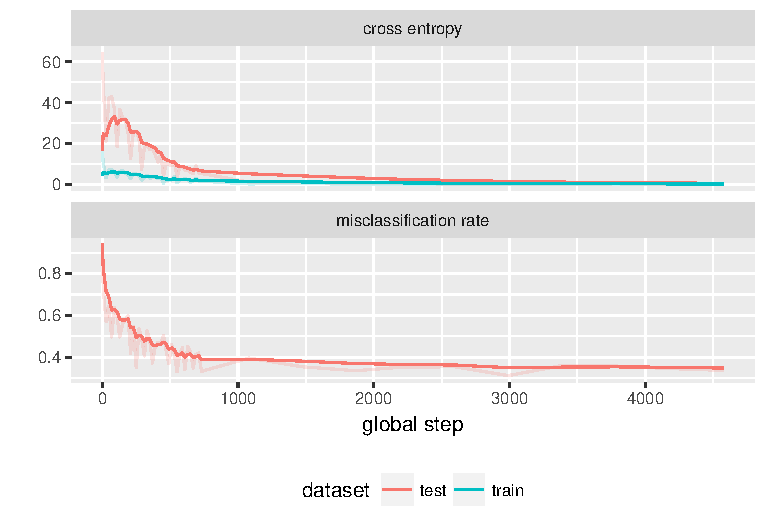
\includegraphics[scale=1]{bytenet/validation-synthetic-digits.pdf}
    \caption{Shows misclassification rate and the cross entropy loss. For comparison an attention model has a misclassification rate of 0.51. The exponential moving average uses a forget factor of $0.1$.}
    \label{fig:result:bytenet:digits}
\end{figure}

\begin{table}[h]
\centering
\begin{tabular}{r|p{3.3cm} p{3.3cm} p{3.3cm}}
	obs. & source & target & prediction\\ \hline
  0 & one zero four & 104 & 104 \\
  1 & one five six & 156 & 150 \\
  2 & five five nine & 559 & 559 \\
  3 & one six & 16 & 68 \\
  4 & two three four & 234 & 235 \\
  5 & five three & 53 & 53
\end{tabular}
\caption{Source, target, and prediction on examples from the test dataset.}
\label{table:result:bytenet:digits}
\end{table}

Figure \ref{fig:result:bytenet:digits} shows reasonable convergence, only the test error shows jitter during training and there is very little overfitting if any. In the end, the ByteNet model completely learned the training dataset.

The jitter is likely not because of poor optimization, but rather because the errors are only calculated on a randomly sampled subset of the test dataset. For the different samples, the test error is thus different.

The lack of overfitting fits well with what the original ByteNet article also observed, in their translation model no regularization or early stopping was used, which is what one would typically use to prevent overfitting \cite{bytenet}.

In table \ref{table:result:bytenet:digits} the predictions are about what one would expect. For the most part, the translations are good, in particular in the beginning of the output sequence, while the later digit predictions show some error. This result is reasonable, as there is more data for the first two digits and because the input words have different lengths. The alignment between input and output characters becomes more uncertain as the read sequences get longer. Of cause, the model would ideally learn the word separation completely and understand that there is a direct relation between word and digit, but learning this relation is likely difficult given both the many parameters and the small dataset.

\clearpage
\subsubsection{Memorizing WMT NewsTest}

Sometimes a model works well when it has few weights and low dimensionality but breaks for higher dimensionality because of vanishing or exploding gradient issues. To validate that this is not an issue a good test is to see if the model can memorize a small dataset, but where the model complexity is kept high. For memorization one just expects the training loss to become very small, the test error is not important.

The WMT 2014 NewsTest dataset for German to English translation was used for training, this contains 3003 observations. The WMT 2015 NewsTest dataset was used for testing, this contains 1596 observations. The internal dimensionality is set to 400, (800 in the decoder because of concatenation).

The model ran 120 epochs over the training dataset, with a mini batch size of ${4 \cdot 16 = 64}$, running on 4 GPUs in parallel using synchronized updates with the Adam optimizer and a learning rate of 0.0003.

\begin{figure}[h]
    \centering
    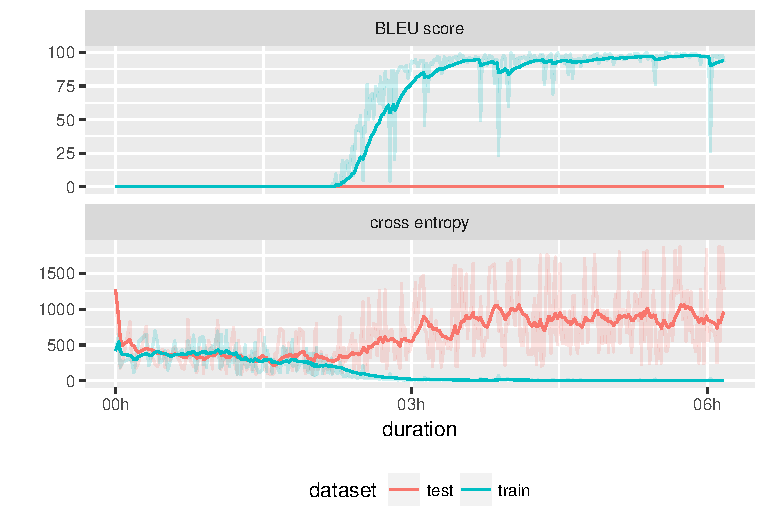
\includegraphics[scale=1]{bytenet/validation-memorize-wmt.pdf}
    \caption{Shows BLEU score and cross entropy loss for the German to English WMT NewsTest dataset. Both training and test measures are calculated on a randomly sampled mini-batch from each dataset. The exponential moving average uses a forget factor of $0.3$.}
    \label{fig:result:bytenet:wmt}
\end{figure}

\begin{table}[h]
\centering
\begin{tabular}{l|r|p{10cm}}
  0 & source & Polizei von Karratha verhaftet 20-Jährigen nach schneller Motorradjagd \\[0.1cm]
    & target & Karratha police arrest 20-year-old after high speed motorcycle chase \\[0.1cm]
    & translation & In must in the ugains of the with of Chanamby a leadn-Minor ald the ace the town of the construction of the compunity the government. \\[0.1cm]
    & BLEU & 0.00 \\[0.1cm] \hline
  1 & source & Das Motorrad wurde sichergestellt und für drei Monate beschlagnahmt. \\[0.1cm]
    & target & The motorcycle was seized and impounded for three months. \\[0.1cm]
    & translation & The New York works with smaries for twe to the come to cover earling scace us deliving the construction work. \\[0.1cm]
    & BLEU & 0.00
\end{tabular}
\caption{Source, target and prediction on the test dataset.}
\label{table:result:bytenet:wmt-test}
\end{table}

\begin{table}[h]
\centering
\begin{tabular}{l|r|p{10cm}}
  0 & source & Demgegenüber unterrichten australische Schulen durchschnittlich 143 Stunden jährlich und Schüler in Singapur erhalten 138 Stunden. \\[0.1cm]
    & target & By comparison, Australian schools provide an average of 143 hours a year and pupils do around 138 hours in Singapore. \\[0.1cm]
    & translation & By comparison, Australian schools provide an average of 143 hours a year and pupils do around 138 hours in Singapore. \\[0.1cm]
    & BLEU & 100.00 \\[0.1cm] \hline
  1 & source & Diese Umlage wird jedes Jahr im Oktober von den vier Betreibern der der großen Stromtrassen neu festgesetzt. \\[0.1cm]
    & target & This levy will be reset by the four operators of the large power grids, in October of each year. \\[0.1cm]
    & translation & This levy will be reset by the four operators of the lerge power grids, in October of each year. \\[0.1cm]
    & BLEU & 87.23
\end{tabular}
\caption{Source, target and prediction on the training dataset.}
\label{table:result:bytenet:wmt-train}
\end{table}

Ensuring that the optimization converges was the primary purpose of this experiment. Figure \ref{fig:result:bytenet:wmt} shows that the parameter optimization does like in the synthetic digits problem, appear to converge just fine. Initially, there is some jitter in the cross entropy training loss, but this subsides after awhile.

In the beginning, the jitter frequency is higher this is just because TensorFlow samples values at fixed time intervals. Initially, there are some allocations and data transfers that causes the model to run slower, thus as a side effect TensorFlow samples more frequently in this period. 

As said the test loss is not very interesting, as there isn't enough training data to expect the model to produce meaningful results. The cross entropy on the test dataset does also show an increase after the initial decrease, which indicates some overfitting. Again, this is to be expected given the small training dataset.

More interesting is the correlation between the training cross entropy and the training BLEU score. Initially, the cross entropy decreases a lot, but the BLEU score stays at 0. It is first when the cross entropy nears 0, that the BLEU score begins to improve. This observation is quite important as it indicates that cross entropy isn't a perfect loss measure for the translation problem. This is because the cross entropy can be quite low if it just gets the majority of the characters almost correct, but the position must be correct. The BLEU score, on the other hand, demands that the words matches exactly, but is looser regarding the position. For example, in table \ref{table:result:bytenet:wmt-train} the target is ``large'' but the prediction is ``lerge''. This is very close in terms of cross entropy but is completely wrong in terms of the BLEU score, since the words don't match. Nevertheless, the cross entropy loss is useful because its gradient in combination with softmax is easily computable, and the BLEU score does become very high in the end, even though the correlation between cross entropy and the BLEU score is weak.

The training BLEU score is actually extremely good, it shows almost a perfect translation. Typically translation models only show a BLEU score between 15 and 25 on a test set. This is not necessarily because the translation is wrong but because there are many different ways of translating a sentence correctly. The BLEU score does actually support multiple target sequences, but this is rarely provided in the test dataset because of the labor demands for creating multiple translations.

The only way the model can be this good is by primarily memorizing the output given the input. It is unlikely there is much understanding of the latent semantic meaning in the text. That being said, the predictions in table \ref{table:result:bytenet:wmt-test} shows that the model understands some grammar, such as which words comes before nouns. That being said, the second prediction example in table \ref{table:result:bytenet:wmt-test} contains a single quotation mark, which is not grammatically meaningful. 

Some of the above-mentioned issues could perhaps be improved by not using the target sequence in the decoder during training step. Instead, the predicted sequence could be used in the decoder input, just like in the inference model. This could solve issues like ``large'' becoming ''lerge''. The disadvantage of doing this is that training would be slower, as the decoder can't be parallelized over the sequence. Some research suggests that one should use a hybrid model, where the training loss is composed of both an assisted part and a non-assisted part, in the latter case the target sequence isn't used \cite{no-assist-train}.

Another observation is that the predicted sequences are in general a bit longer than the target sequences. This is likely because of how the sequence loss is constructed, this only measures the error where the target is explicitly known. Thus there is little penalty for predicting longer sequences than the target sequence. However, there is some penalty, because the predicted \texttt{<eos>} symbol should match the target \texttt{<eos>} symbol. More penalty could be added by padding the target sequence sufficiently with a special \texttt{<null>} symbol, and then also measure the error on that part of the sequence. However, this introduces an issue where the translation model can just predict ``\texttt{<null><null><null><null>...}'' and this will in terms of cross entropy be a good match since the majority of the sequence matches. This is an easily obtainable solution for the optimizer, it can thus be a local minimum that is difficult to escape.

\clearpage
\subsection{WMT Translation Task}

With the ByteNet model reasonably validated in terms of generalization on the synthetic digits problem, and convergence when memorizing the WMT NewsTest dataset, the ByteNet model is used on the Europarl v7 dataset for German to English translation.

\begin{figure}[h]
    \centering
    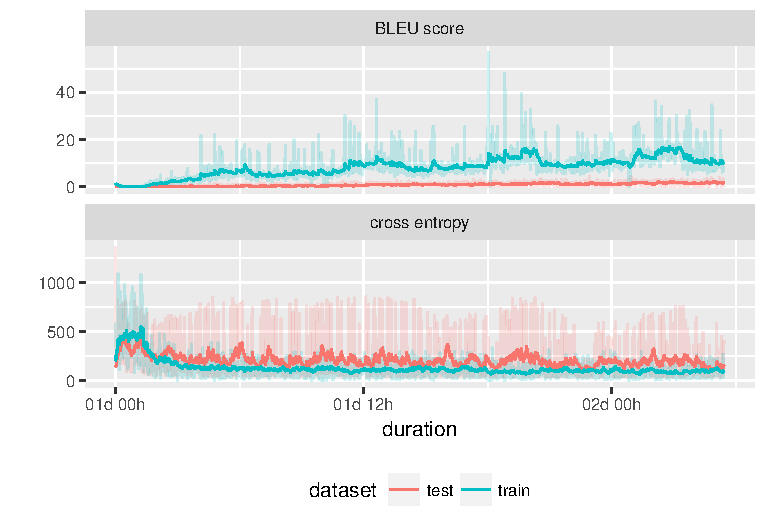
\includegraphics[scale=1]{bytenet/europarl.pdf}
    \caption{Shows BLEU score and cross entropy loss for ByteNet, trained on Europarl v7 and tested on WMT NewsTest 2015. Both training and test measures are calculated on a randomly sampled mini-batch from each dataset. The exponential smoothing uses a forget factor of $0.05$. The vertical lines separates each batch epoch.}
    \label{fig:result:bytenet:europarl}
\end{figure}

The ByteNet model has an internal dimensionality of 400, just like the model used for training on the WMT NewsTest dataset. The Adam optimizer with a learning rate of 0.0003 is used for training. This used a training mini-batch size of $4 \cdot 16 = 64$ observations and the model was trained on 4 GPUs in parallel with synchronized updates. The Europarl v7 dataset is used for training and the training ran 13 epochs over the Europarl v7 dataset. The WMT NewsTest 2015 dataset is used for testing, the continues testing was done on randomly sampled mini-batches with 128 observations each.

From figure \ref{fig:result:bytenet:europarl} it's seen that the BLEU score on the test dataset is approximately $5.5$. However, because that BLEU score is calculated on a random subset of the dataset it is not completely accurate. The actual BLEU score calculated on the entire WMT NewsTest dataset after training is $7.44$. The translations are shown in table \ref{table:result:bytenet:high-belu} and table \ref{table:result:bytenet:zero-belu}.

Figure \ref{fig:result:bytenet:europarl} also shows some oscillation that is correlated with the epochs. After further investigation it turns out that there are bad translations in the dataset, some examples can be seen in table \ref{table:result:bytenet:bad-translations}. Such observations would misdirect the optimization in each epoch and thus cause oscillation. However, even after removing all observations with either a source or target sequence less than 25 characters, the oscillation still exists. Given that the oscillation is correlated with the epochs, it is most likely the dataset that still contains poor observations. However, finding these among 2 million sentence pairs is rather difficult, a possible solution could be to increase the bucket size, such that there is a higher probability for the poor translations to be mixed with the good translations in each mini-batch.

\begin{table}[h]
\centering
\begin{tabular}{l|r|p{10cm}}
0 & source & Herr Kommissar! \\[0.1cm]
  & target & \\[0.1cm] \hline
2 & source & \\[0.1cm]
  & target & There are, therefore, two points to which I would like to draw the Commission' s attention. \\[0.1cm]  \hline
3 & source & \\[0.1cm]
  & target & This is something about which European small and medium-sized businesses, in particular, tend to complain.
\end{tabular}
\caption{Examples of bad translations in the Europarl v7 dataset.}
\label{table:result:bytenet:bad-translations}
\end{table}

\begin{table}[h]
\centering
\begin{tabular}{l|r|p{10cm}}
0 & source & Die formelle Anerkennung der Arbeitsrechte als Menschenrechte - und die Erweiterung des Schutzes der Bürgerrechte als Schutz gegen Diskriminierung bei der Schaffung von Arbeitnehmervertretungen - ist längst überfällig. \\[0.1cm]
& target & The formal recognition of labor rights as human rights - and the extension of civil rights protections to prevent discrimination against labor organizing - is long overdue. \\[0.1cm]
& translation & The formal recognition of human rights as human rights - and the extension of the protection of civil liberties as a protection against discrimination against employment organizations - is long overdue. \\[0.1cm]
& BLEU & 45.97 \\[0.1cm] \hline

1 & source & Aber es ist mit Sicherheit keine radikale Initiative - jedenfalls nicht nach amerikanischen Standards. \\[0.1cm]
& target & But it in certainly not a radical initiative - at least by American standards. \\[0.1cm]
& translation & But it is certainly not a radical initiative, at least for American standards. \\[0.1cm]
& BLEU & 39.13 \\[0.1cm] \hline

2 & source & Das Militär spielt in Pakistan eine wichtige Rolle und hat bereits häufiger geputscht. \\[0.1cm]
& target & The military plays an important role in Pakistan and has taken power by force several times in the past. \\[0.1cm]
& translation & Military players play an important role in Pakistan and has already been developing more and more. \\[0.1cm]
& BLEU & 30.18
\end{tabular}
\caption{Cherry-picked translations from WMT NewsTest with high BLEU score.}
\label{table:result:bytenet:high-belu}
\end{table}

\begin{table}[h]
\centering
\begin{tabular}{l|r|p{10cm}}
0 & source & Die Premierminister Indiens und Japans trafen sich in Tokio. \\[0.1cm]
& target & India and Japan prime ministers meet in Tokyo \\[0.1cm]
& translation & The Prime Minister of India and Japan worked in Tokyo. \\[0.1cm]
& BLEU & 0.00 \\[0.1cm] \hline

1 & source & Er wird beschuldigt, am 7. Juni 2013 eine Frau im Scotland's Hotel in Pitlochry in Perthshire vergewaltigt zu haben. \\[0.1cm]
& target & He is alleged to have raped a woman at the Scotland's Hotel in Pitlochry in Perthshire on June 7, 2013. \\[0.1cm]
& translation & He is accused of being a Member of the European Parliament in Scotland in Petersberg in Peru. \\[0.1cm]
& BLEU & 0.00 \\[0.1cm] \hline

2 & source & Angelina Jolie und ihr Bruder James haben eine Videohommage für ihre Mutter online gestellt, die 2007 an Eierstockkrebs verstarb. \\[0.1cm]
& target & Angelina Jolie and her brother James have posted a video tribute to their late mother who died of Ovarian cancer in 2007. \\[0.1cm]
& translation & Angela John and her village of James have created violence for their mother-tongue, which involves emergency catastrophe. \\[0.1cm]
& BLEU & 0.00 \\[0.1cm] \hline

3 & source & "Diese Krankheit wird am besten von gynäkologischen Onkologen behandelt, und diese sind meistens in größeren Städten zu finden," sagte sie. \\[0.1cm]
& target & "This disease is best treated by gynaecological oncology surgeons and they're mostly based in major cities," she said. \\[0.1cm]
& translation & 'This disease is best achieved by organic chocolate industries, and these are indeed more than "more cities'. \\[0.1cm]
& BLEU & 0.00
\end{tabular}
\caption{Cherry-picked translations from WMT NewsTest with zero in BLEU score.}
\label{table:result:bytenet:zero-belu}
\end{table}

Looking at the actual translations, those with a high BLEU score in table \ref{table:result:bytenet:high-belu} are as expected quite good. Much more interesting is to look at the bad translations in table \ref{table:result:bytenet:zero-belu}.

Translation \texttt{0} is actually a very good translation, but the different word ordering means that it gets a BLEU score of zero. This is an example of the BLEU score not always being a good measurement of text similarity.

Translation \texttt{1} is on the other hand quite bad, except for the ``He is accused'' part it is very wrong. It is apparent that the translation model detects places by its initial capital letter and attempts to translate these but the translations are rarely correct. This is quite interesting since translating names should often be easy since it is just the identity function. However, such a mapping requires the model to switch between a semantic understanding and the identity function. This behavior may be difficult for the model to learn as it will initially either learn semantic understanding or the identity function. Once that is partially learned the model will use its entire parameter space for that purpose. Compressing this parameter space and allowing for a new mode of operation is perhaps not a likely gradient direction in the optimization, as more would initially be lost by the compression than what is gained by the extra mode. That being said character-based models have been shown to be able to learn this behavior \cite{character-alignment}.

Translation \texttt{1}, \texttt{2}, and \texttt{3} are all interesting because while the translations may be bad the grammatical part is mostly fine. This indicates that the model understands basic language constructs. An example is that ``He is accused of being a Member of the European Parliament'' makes sense even though the translation is very wrong.

\clearpage
\subsection{Performance profiling}
The ByteNet model is rather slow. For ByteNet to reach a BLEU score of 23 as Google achieved in the original paper, it will have to train on a much bigger dataset for much a longer time.

\begin{figure}[h]
    \centering
    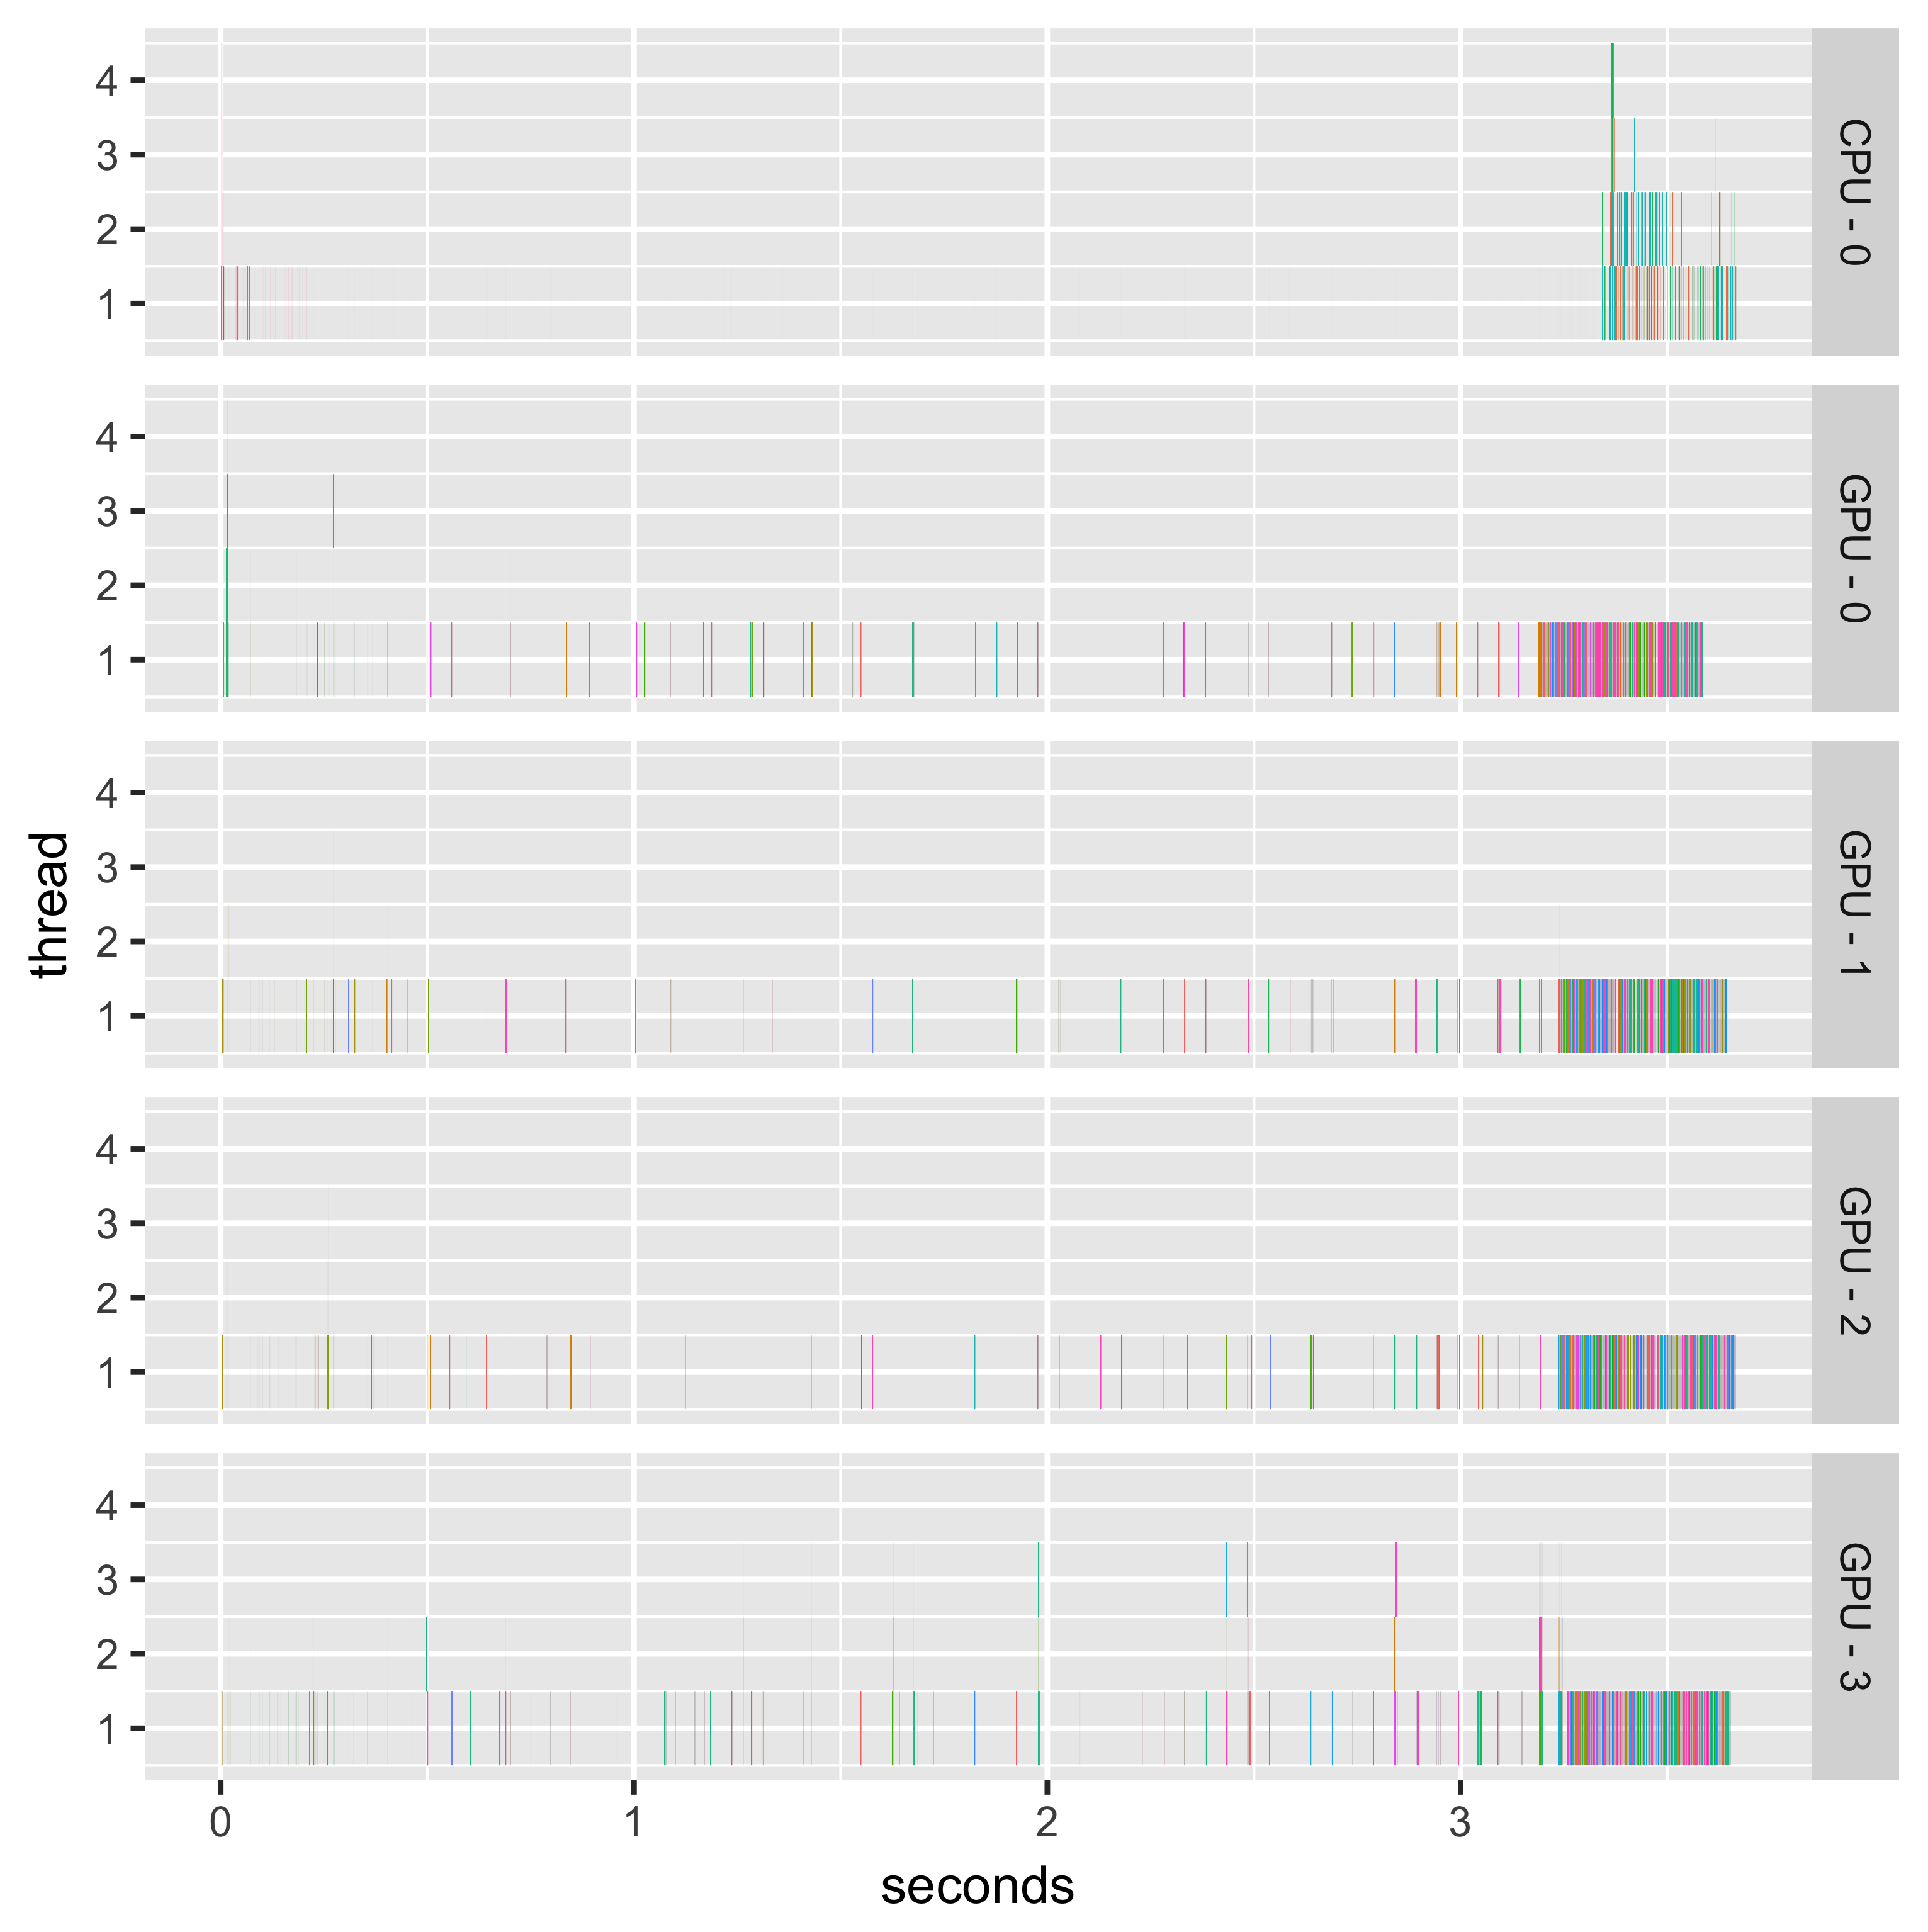
\includegraphics[width=\textwidth]{bytenet/profile-raw-gpu4.png}
    \caption{Shows time spent on each operation, when the operation was executed, and on what GPU/CPU it was executed. The color coding indicates the operation type, there are more than a 100 different operation types, most are specific to TensorFlow, thus the legend is not included.}
    \label{fig:result:bytenet:profile-raw}
\end{figure}

To understand why the ByteNet model is so slow, TensorFlow was profiled while executing the computational graph. The setup is identical to the ``Memorizing WMT NewsTest'' setup running on 4 GPUs, and the profiling was done when evaluating the 4500th mini-batch. The 4500th mini-batch was chosen because the performance has reached its peak and stabilized.

From figure \ref{fig:result:bytenet:profile-raw} it's seen that most of the time is not spent computing, but rather waiting for data to be transferred or just waiting for the TensorFlow service to queue a new task.

\begin{figure}[h]
    \centering
    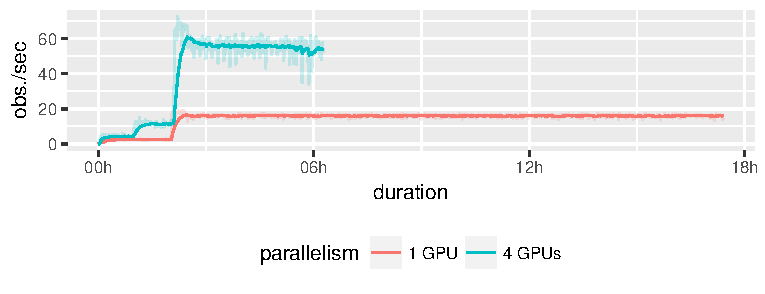
\includegraphics[scale=1]{bytenet/timing-gpus.pdf}
    \caption{Comparing observations per second, depending on the number of GPUs used.}
    \label{fig:result:bytenet:timing-gpus}
\end{figure}

By comparing the speed of how fast the ByteNet implementation processes observations, depending on the number of GPUs used, one gets that about 37\% of the time is spent waiting for data transference in the 4 GPUs case. This calculation does, in particular, make sense when comparing with 1 GPU, since a 1 GPU setup will not require data transfer of any weights. This is because the gradients and weights don't need to be synchronized on the CPU, but can be kept on the GPU where they are calculated.

The data transfer does not explain all the waiting time. Likely this particular profiling is an extreme case. TensorFlow transfers the dataset in chunks in preparation for future mini-batches. If TensorFlow is transferring the dataset while profiling in this exact moment, that will cause extra waiting time.

By processing the profiling dump file, such that the waiting time is removed from the data, one can see that time is primarily spent in the layers that contain normalization and activation (\textit{pre-normalization}, \textit{conv-dilated}, \textit{reduce-dim}).

\begin{figure}[h]
    \centering
    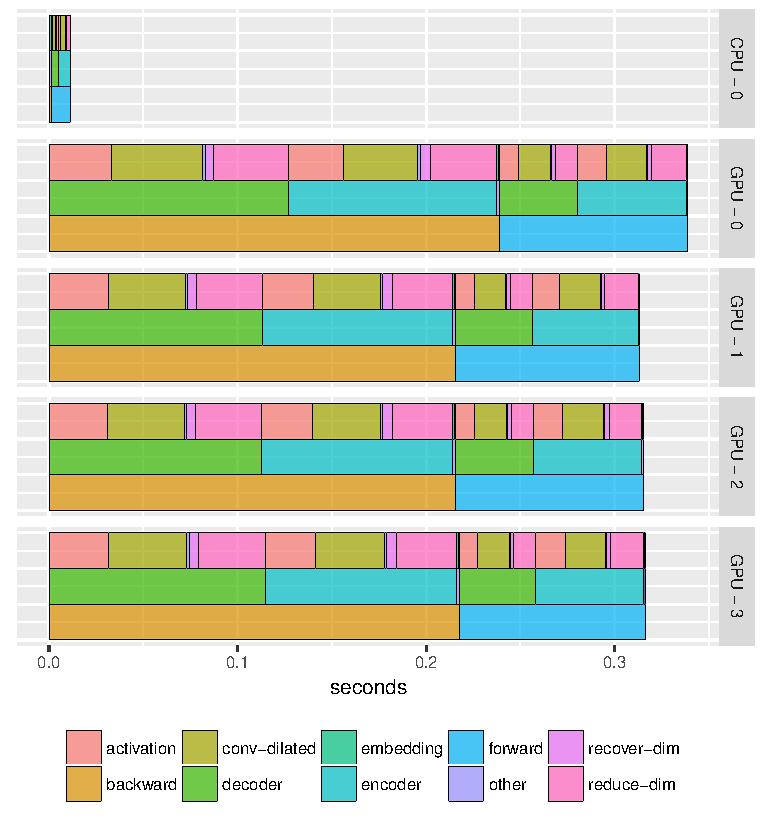
\includegraphics[scale=1]{bytenet/profile-grouped-gpu4.pdf}
    \caption{Shows time spent executing each part of the ByteNet model, this excludes the waiting time. Each part exists in a hierarchy, which is visualized as levels. Bottom level is the backward and forward pass. Second level is the encoder and decoder. Last level primarily splits the ByteNet Residual Blocks.}
    \label{fig:result:bytenet:profile-grouped}
\end{figure}

It is likely that the data transfer part could be optimized, but in general, this isn't easy and there are practical limitations to how much it can be improved. It is much more likely that the waiting time regarding the TensorFlow service could be improved.

TensorFlow works with a computational graph. Each atomic operation, like an element-wise addition or a matrix multiplication, is a node in this graph and the edges describe the dependencies. The TensorFlow service will watch the graph and execute any node (atomic operation) when all its dependencies are satisfied, it will even execute multiple nodes in parallel if possible. This process repeats until all nodes have been computed and the end result is obtained.

Using a computational graph is a good strategy, but the current TensorFlow implementation of it is very naive. TensorFlow uses no-op and identity operations, which only exists because of TensorFlow semantics, but don't need to be executed. However, in the current state of TensorFlow, it just executes all nodes naively. There are also numerous of atomic operations that could be fused into one atomic operation. An example is batch normalization that involves quite a few element-wise operations, all these are executed separately but could be combined into a single atomic operator. All these atomic operators are what causes the waiting time, the TensorFlow service needs to walk the computational graph and more importantly just launching GPU kernels also introduces wasted time.

The TensorFlow team is aware of the current limitations and are in the process of solving these issues, by using a Just In Time compiler that can automatically fuse many of these operations. But so far this is in an experimental state and performs very poorly when running on multiple GPUs \cite{google-xla}.

\clearpage

\section{Simplified ByteNet}

The implementation of the ByteNet model spends $37\%$ of its time waiting for data transfer between GPU and CPU and even more time waiting on the TensorFlow service. This is because of the large amount of weights and operations that is used in the ByteNet model.

To solve this issue a simplified version of ByteNet has been created. This uses less weights and less operations than ByteNet, but remain true to principals behind ByteNet. Those principals is running in linear time, parallelize over both sequence and observations, have be resolution persistent meaning that the size of the encoded representation scales with the sequence length. The simplified version also maintains the bottleneck of 200 dimensions that ByteNet has in its dilated-convolution layer.

The idea behind this is simple, if the initial embedding dimensionality is set to 200 then the compression and decompression layers that exists before and after the dilated convolution are not needed. Of cause these layers adds non-linearities and weights to the model, thus one should not expect the model to perform equally well. Instead the model should before almost as well and be significantly faster.

\begin{figure}[H]
    \centering
    \begin{subfigure}[b]{0.45\textwidth}
        \centering
        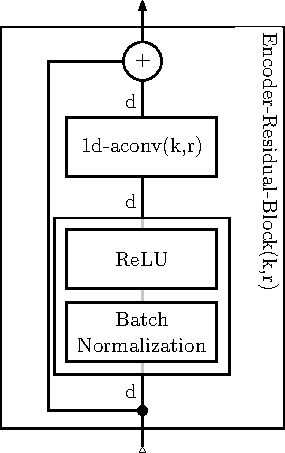
\includegraphics[scale=1]{theory/bytenet-small-residual-block.pdf}
        \caption{Residual Block used in encoder.}
    \end{subfigure}
    ~ %
    \begin{subfigure}[b]{0.45\textwidth}
        \centering
        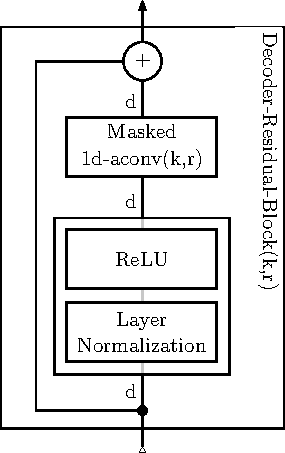
\includegraphics[scale=1]{theory/bytenet-small-residual-block-causal.pdf}
        \caption{Residual Block used in decoder.}
    \end{subfigure}
    \caption{The residual blocks used in the Simplified ByteNet model. The blocks are denoted by Encoder-Residual-Block$(k,r)$ and Decoder-Residual-Block$(k,r)$, where $k$ is the kernel width and $r$ is the dilation rate.}
    \label{fig:result:simple-bytenet:residual-block}
\end{figure}

In terms of weights the simplified ByteNet model has approximately $\sfrac{5}{9}$ times less weights than the ByteNet model. The simplified ByteNet model also has approximately one third of the operations as the ByteNet model. Based on these parameters one should expect less transfer time and less time spend waiting for the TensorFlow service.

The simplified ByteNet model was validated identically to the how the ByteNet model was validated. The results (appendix \ref{appendix:result:bytenet-small}) where very similar with some minor differences. Memorizing WMT NewsTest took fewer iterations, this is likely because there are fewer parameters. The simplified ByteNet model learned the synthetic digits problem better, with a misclassification error of $0.25$. An explanation could for the improved misclassification error is that the the simplified ByteNet model has fewer parameters and non-linear transformation, this might make it overfit less.

\subsection{Performance Profiling}

To compare the performance of the simplified ByteNet model with the normal ByteNet model, the performance experiment from the normal ByteNet model was repeated using the simplified ByteNet model. This experiment learns the WMT NewsTest dataset over 300 epochs. Both a 1 GPU and a 4 GPU setup was used in the experiments.

\begin{figure}[h]
    \centering
    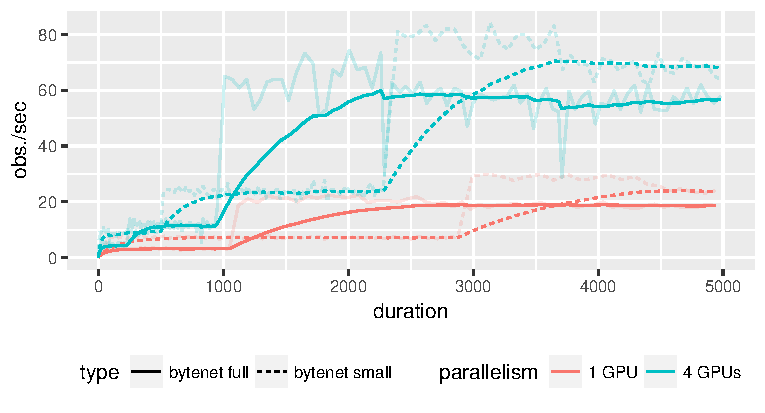
\includegraphics[scale=1]{bytenet-small/timing-gpus.pdf}
    \caption{Comparing observations per second, depending on the number of GPUs used.}
    \label{fig:result:simple-bytenet:timing-gpus}
\end{figure}

Measuring the total time spend and the observations per second as seen in figure \ref{fig:result:simple-bytenet:timing-gpus} reveals that the simplified ByteNet model is faster. On 1 GPU the simplified ByteNet model is about $20\%$ faster. This is quite far from the best case $66\%$, that one would get from reducing the number of operation to $\sfrac{1}{3}$.

On 1 GPU there is no data transfer, thus it is only the TensorFlow service and the computation that takes time. Assuming the actual computation time is not the most time consuming part, reducing the number of operations to $\sfrac{1}{3}$ should result in a $\sfrac{2}{3}$ computational performance gain. This is of cause an approximation as there is still the embedding layer, the concatenation of encoding and decoding, and the final output layer, thus $\sfrac{2}{3}$ the operations is an upper bound.

Comparing the time spend in the 1 GPU experiment and the 4 GPU experiment, and because very little data transfer happens when using 1 GPU. The data shows that approximately $40\%$ time is spend transferring data. This is approximately the same as the $37\%$ in the normal ByteNet model. The number of weights is reduced by $\sfrac{5}{9}$, thus one would expect the transfer time to be reduced by this order, however that is not the case.

\begin{figure}[h]
    \centering
    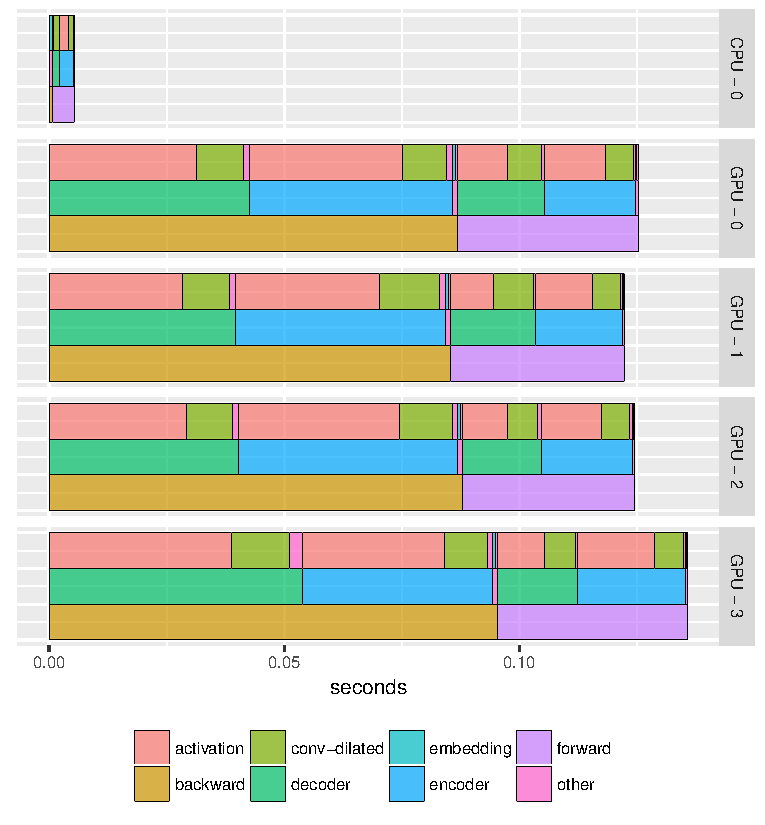
\includegraphics[scale=1]{bytenet-small/profile-grouped-gpu4.pdf}
    \caption{Shows time spend executing operations in each part of the ByteNet model, this excludes the waiting time. Each part exists in a hierarchy, which is visualized as levels. The bottom level is the least detailed level, it just splits the model in the backward and forward pass. The next level, splits the model in the encoder and decoder. The last level at the top, primarily splits the Simplified ByteNet Residual Blocks.}
    \label{fig:result:simple-bytenet:profile-grouped}
\end{figure}

Finally the TensorFlow profiler can be used to investigate what takes time. When processed the results are similar to those from the normal ByteNet model, see figure \ref{fig:result:simple-bytenet:profile-grouped}.

From figure \ref{fig:result:simple-bytenet:profile-grouped} that much of the time is spend in the \textit{activation layer}. The \textit{activation layer} is the layer that contains the normalization and ReLU operation. This validates the idea that it is the number of operations and not the operations themselves that cost in terms of time. The dilated convolution (called \textit{conv-dilated}) is a much more complex operation than normalization or ReLU, but TensorFlow implements it using just a few operations, thus it doesn't consume that much time. As mentioned earlier the TensorFlow team is aware of this performance issue, and tries to solve it my automatically compiling GPGPU (CUDA or OpenCL) kernels that combines multiple operations into one, but this is still very experimental and doesn't yet provide a performance when using multiple GPUs \cite{citation-needed}.

\clearpage
\subsection{WMT Translation Task}

The Europarl v7 dataset is used to train the simplified ByteNet model. The setup is identical to that previously used to train the normal ByteNet model. The internal dimensionality is 400, the Adam optimizer is used with a learning rate of 0.0003, and the mini-batch size is $4 \cdot 16 = 64$ observations, 4 GPUs with synchronized updates was used, and the model ran 13 epochs over the Europarl v7 dataset.

\begin{figure}[h]
    \centering
    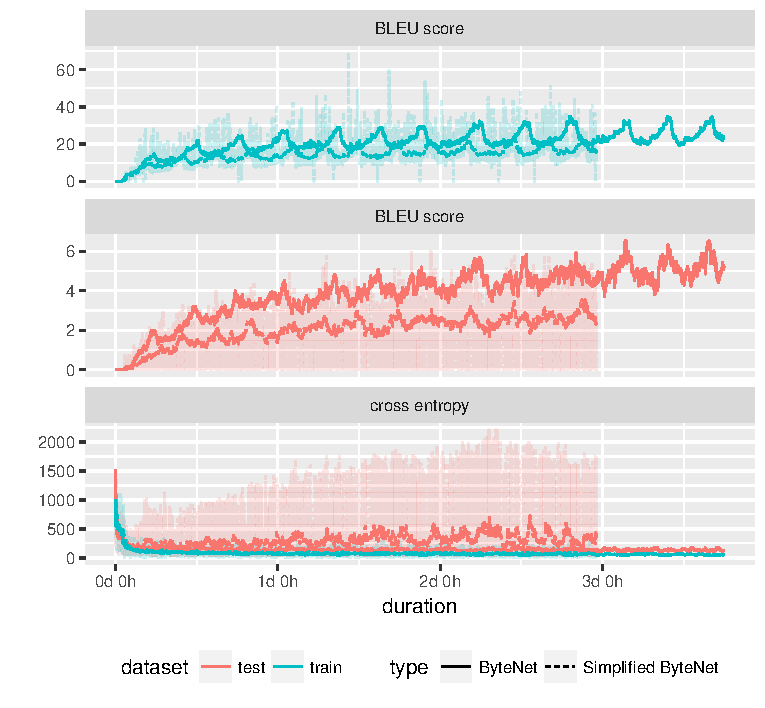
\includegraphics[scale=1]{bytenet-small/europarl.pdf}
    \caption{Shows BLEU score and cross entropy loss for the Simplified ByteNet model, trained on Europarl v7 and tested on WMT NewsTest 2015. Both training and test measures are calculated on a randomly sampled mini-batch from each dataset. The exponential smoothing used a forget factor of $0.05$. The raw data for the non-simplified ByteNet model is not shown.}
    \label{fig:result:bytenet-small:europarl}
\end{figure}

The simplified ByteNet model uses almost 24 hours less training time. However, it also learns at a slower rate, thus in terms of BLUE score given the time spend learning the normal ByteNet model is actually much faster.

An interesting observation is that the simplified ByteNet model also overfits a lot more than the normal ByteNet model. This contradicts most intuition about overfitting, which usually is the more weights, layers, and non-linearities, the easier it is to make the model overfit. The simplified ByteNet model has less of all three factors, thus there is no reason to expect the simplified ByteNet model to overfit more.

It is not clear why this overfitting happens, but it is very likely a contributing factor to why the test BLEU score isn't isn't better. However, this can not be the entire explanation, as also the training BLEU score is worse. If anything, overfitting should cause a higher training BLEU score as regularization typically increases the training loss in order to decrease the test loss.

Possible regularization methods are L1, L2, and dropout. Particularly, L1 regularization could be interesting in the first 5 \textit{residual blocks}, as these layers likely performs some characters-to-word encoding. Such an encoding should be very sparse, L1 regularization would enforce such a sparsity.

The translations as shown in table \ref{table:result:bytenet-small:translations} are rather bad, they have little connection to the source sequence and there a tendency for the sequence ``Mr \textit{insert name}'' to appear without context. The poor translations can likely be attributed to the server overfitting. \todo{total BLEU score is $0.55$}

\begin{table}[h]
\centering
\begin{tabular}{l|r|p{10cm}}
0 & source & Die formelle Anerkennung der Arbeitsrechte als Menschenrechte - und die Erweiterung des Schutzes der Bürgerrechte als Schutz gegen Diskriminierung bei der Schaffung von Arbeitnehmervertretungen - ist längst überfällig. \\[0.1cm]
& target & The formal recognition of labor rights as human rights - and the extension of civil rights protections to prevent discrimination against labor organizing - is long overdue. \\[0.1cm]
& translation & However, the recommendation of jobs and generations and proposes the promotion of gross regions of the world growth to prodictively rejecting the rejection of the representative of the representative increase' . \\[0.1cm]
& BLEU & 0.00 \\[0.1cm] \hline

1 & source & Die Premierminister Indiens und Japans trafen sich in Tokio. \\[0.1cm]
& target & India and Japan prime ministers meet in Tokyo \\[0.1cm]
& translation & Mr Pieper and the independence of Singapore in London. \\[0.1cm]
& BLEU & 0.00 \\[0.1cm] \hline

2 & source & Er wird beschuldigt, am 7. Juni 2013 eine Frau im Scotland's Hotel in Pitlochry in Perthshire vergewaltigt zu haben. \\[0.1cm]
& target & He is alleged to have raped a woman at the Scotland's Hotel in Pitlochry in Perthshire on June 7, 2013. \\[0.1cm]
& translation & Madam President, I should like to contribute to Mr President Mr President in his report. \\[0.1cm]
& BLEU & 0.00 \\[0.1cm]
\end{tabular}
\caption{Cherry-picked translations from WMT NewsTest.}
\label{table:result:bytenet-small:translations}
\end{table}


\clearpage

\section{SELU ByteNet}

The Simplified ByteNet experiments indicates that, the compression and decompression layers are necessary, and the normalization layers are very expensive. From these observations it makes sense to analyse whether the normalization layers are actually necessary for the network to converge.

The experiment in figure \ref{fig:result:selu-bytenet:bytenet-nonorm-wmt} is the ``Memorizing WMT NewsTest'' experiment on the ByteNet model without normalization layers. The experiment ran for 300 epochs.

\begin{figure}[h]
    \centering
    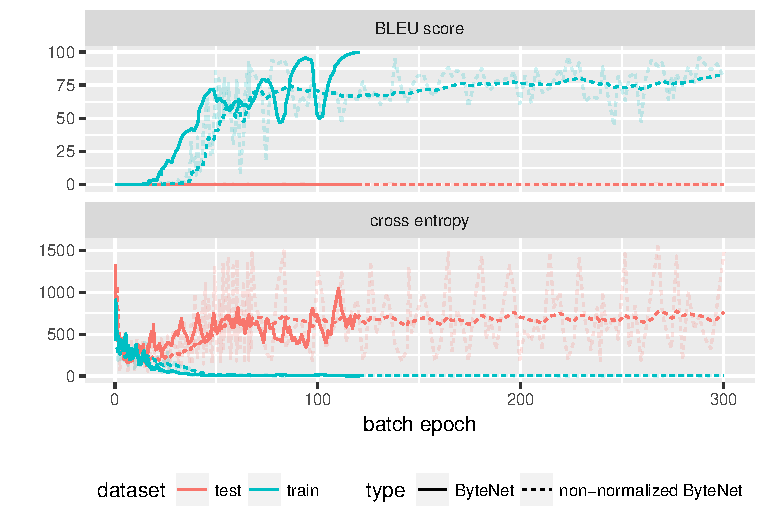
\includegraphics[scale=1]{bytenet-nonorm/validation-memorize-wmt.pdf}
    \caption{Shows BLEU score and cross entropy loss for the German to English WMT NewsTest dataset using the ByteNet model without any normalization layers. The exponential moving average used a forget factor of $0.1$.}
    \label{fig:result:selu-bytenet:bytenet-nonorm-wmt}
\end{figure}

Figure \ref{fig:result:selu-bytenet:bytenet-nonorm-wmt} shows that the non-normalized ByteNet model never completely memorizes the training dataset as it should. It is possible that it could still learn actual translation when trained on the Europarl v7 dataset, however, it is not very likely.

Recently a new paper showed that it is possible to create a ``self-normalizing neural network''. This means that normalization isn't done explicitly by a normalization layer, but instead the network is created such that the parameters will convergence to weights that ensures normalized internal values.

The ``self-normalizing neural network'' was achieved by using a different activation function and weight initialization. Primarily it is the activation function that is responsible for making the network \textit{self-normalizing}, the initialization is primarily just to ensure a reasonable starting point \cite[https://arxiv.org/pdf/1706.02515.pdf]{selu}.

The activation function is a variation on the exponential-linear-unit (ELU), which is similar to the ReLU activation function. The difference is that two constants ($\lambda, alpha$) are added:
\begin{equation}
\mathrm{SELU}(x) = \lambda \begin{cases}
  x & x > 0 \\
  \alpha (\mathrm{exp}(x) - 1) & x \le 0
\end{cases},\quad \text{where: } \begin{array}{c}
  \alpha = 1.6732632423 \\
  \lambda = 1.0507009873
\end{array}
\end{equation}

\todo[inline]{show figure of the SLEU(x) model.}

The initialization should then be done such that $\mathbb{E}[z_{h_\ell}] = 0$ and $\mathrm{var}[z_{h_\ell}] = 1$. This is achieved by initializing the weights such that:
\begin{equation}
\mathrm{Var}[w_{h_{\ell-1}, h_{\ell}}] = \frac{1}{H_{\ell-1}} \quad \Rightarrow \quad r = \sqrt{\frac{3}{H_{\ell-1}}}
\end{equation}
where $r$ is the symmetric uniform distribution parameter, similarly to that used in He-Initialization.

Using the SELU activation function and its derived initialiser, the convergence for the ``Memorizing WMT NewsTest'' experiment is somewhat similar to the normal ByteNet case (figure \ref{fig:result:selu-bytenet:bytenet-selu-wmt}). However, there are some significant differences. The initial cross entropy loss is much higher in the SELU ByteNet case, this indicates that the derived initialiser isn't the optimal choice. Secondly the training BELU score shows almost no improvement initially and then a very fast improvement after a few 75 epochs. These two observations are likely connected, if the initialization is bad it will take a long time for the network to reach a similar state as the normal ByteNet model does initially. If this is true, and if it's possible to initialize the SELU ByteNet model better, the SELU ByteNet model should actually converge in much fewer iterations that the normal ByteNet model.

\begin{figure}[h]
    \centering
    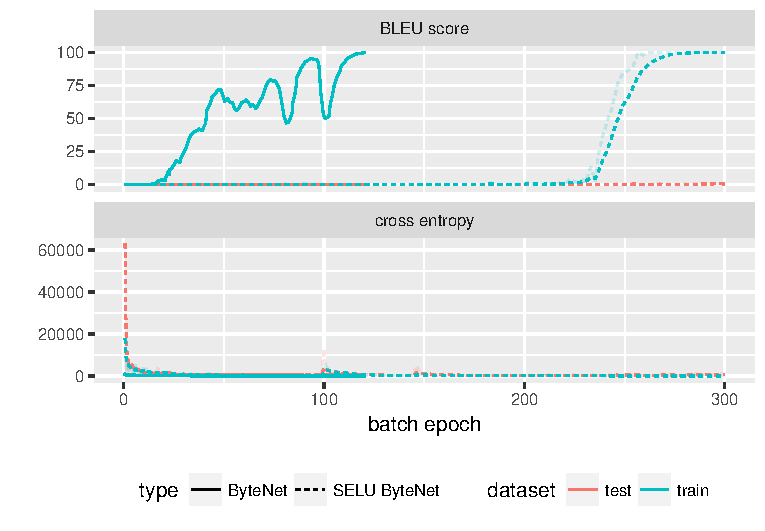
\includegraphics[scale=1]{bytenet-selu/validation-memorize-wmt.pdf}
    \caption{Shows BLEU score and cross entropy loss for the German to English WMT NewsTest dataset using the SELU ByteNet. The exponential moving average used a forget factor of $0.1$.}
    \label{fig:result:selu-bytenet:bytenet-selu-wmt}
\end{figure}

Finally the synthetic digits experiment shows similar results as the normal ByteNet model (Appendix \ref{appendix:result:bytenet-selu}).

\clearpage
\subsection{Performance Profiling}

Repeating the performance experiment from both the normal ByteNet model and the simplified ByteNet model, shows that the SELU ByteNet model is extremely fast in comparison. Comparing the time spend running 300 epochs is actually a problem in this case, as the heating phase that transfers data and optimizes allocation takes up most of the time. However, comparing obs./sec shows that the SELU model is at least twice as fast as the normal ByteNet model.

\begin{figure}[h]
    \centering
    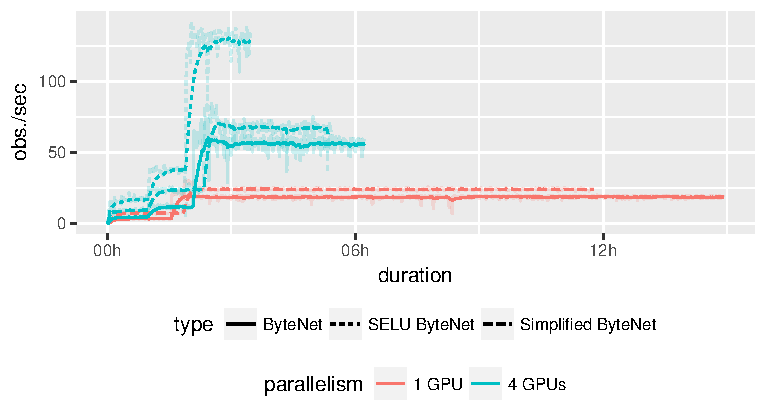
\includegraphics[scale=1]{bytenet-selu/timing-gpus.pdf}
    \caption{Comparing observations per second, depending on the number of GPUs used. The experiment learns the WMT NewsTest dataset over 300 epochs.}
    \label{fig:result:selu-bytenet:timing-gpus}
\end{figure}

The processed profiling in figure \ref{fig:result:selu-bytenet:profile-grouped} (the unprocessed plot is in appendix \ref{appendix:result:bytenet-selu}), shows that the convoluted dilation is the most expensive part. This is completely reasonable, as this is the operation that involves the largest amount of raw computation. However, TensorFlow actually has an inefficient implementation of the dilated convolution, because dilated convolution isn't supported directly by CuDNN v5.1. CuDNN stands for CUDA Deep Neural Network and is a library developed by Nvidia that contains efficient implementation of common operations used in neural networks. The next version of CuDNN supports dilated convolution, but TensorFlow does not yet use this version \cite{nvidia-cudnn}.

Another interesting observation when looking at the processed profiling in figure \ref{fig:result:selu-bytenet:profile-grouped}, is the time spend in the ``\textit{pre-normalization}'' layer, which now just contains the SELU activation, compared to the time spend in \textit{recover-dim}, which just contains a \textit{sequential-dense} layer. This shows that the SELU activation uses an unreasonable amount of time. The SELU activation uses less raw computations than the \textit{sequential-dense} layer, and the SELU activation is purely an element-wise operation and should thus be easy to parallelize. The reason for this performance is the before-mentioned naive execution of the computational graph.

\begin{figure}[h]
    \centering
    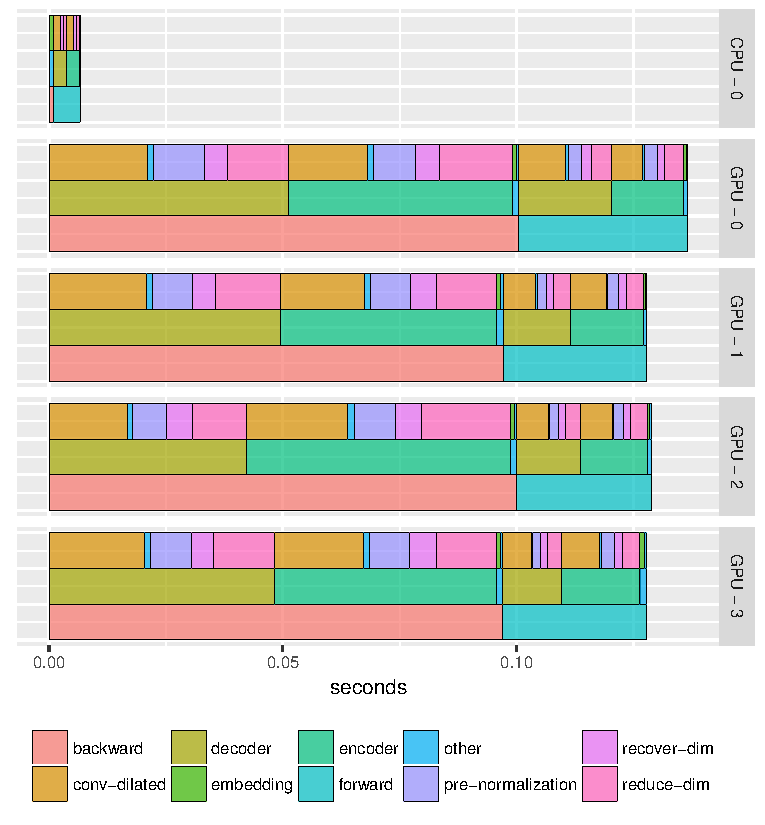
\includegraphics[scale=1]{bytenet-selu/profile-grouped-gpu4.pdf}
    \caption{Shows time spend executing each part of the ByteNet model, this excludes the waiting time. Each part exists in a hierarchy, which is visualized as levels. Bottom level is the backward and forward pass. Second level is the encoder and decoder. Last level primarily splits the SELU ByteNet Residual Blocks.}
    \label{fig:result:selu-bytenet:profile-grouped}
\end{figure}

\clearpage
\subsection{WMT Translation Task}

The Europarl v7 dataset is used to train the SELU ByteNet model. The setup is identical to that previously used to train the normal and simplified ByteNet model.

\begin{figure}[h]
    \centering
    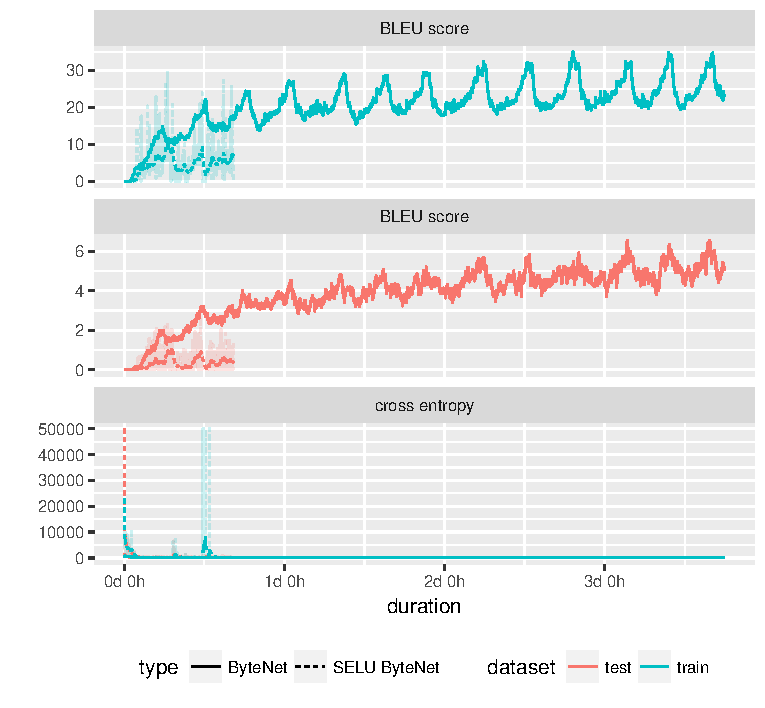
\includegraphics[scale=1]{bytenet-selu/europarl.pdf}
    \caption{Shows BLEU score and cross entropy loss for the SELU ByteNet model, trained on Europarl v7 and tested on WMT NewsTest 2015. Both training and test measures are calculated on a randomly sampled mini-batch from each dataset. The exponential smoothing used a forget factor of $0.05$. The raw data for the non-simplified ByteNet model is not shown.}
    \label{fig:result:bytenet-selu:europarl}
\end{figure}

From figure \ref{fig:result:bytenet-selu:europarl} it is very apparent that the SELU model is extremely fast in comparison to the normal ByteNet model. However it also leans extremely poorly. 

\clearpage


\section{Semi-Supervised ByteNet}

The ``Semi-Supervised Learning for NMT \ref{sec:theory:semi-supervised}'' theory section describes a general idea doing semi-supervised learning in neural machine translation. The method described does not depend on a specific machine learning architecture, but can in theory work using any supervised translation model.

The semi-supervised ByteNet model combines the generalized ``Semi-Supervised Learning for NMT'' ideas with the supervised ByteNet model.

\subsection{Synthetic Digits Problem}

The ByteNet model in itself is rather slow at learning, at least given the current state of TensorFlow. The strategy presented in ``Semi-Supervised Learning for NMT'' does not make this any better. In fact, because the unsupervised part of the loss requires inference using a beam search, the execution time will increase linearly with respect to the beam size. The situation may be even worse for ByteNet since ByteNet when used supervised allows for full palatalization over both the source and target sequence. When inference is done on the ByteNet model, as it is in the unsupervised case, only the encoder part is supervised.

Because of these complications, it is not feasible to apply the Semi-Supervised ByteNet model on the full Europarl v7 dataset and another monolingual (unlabeled) dataset. Instead, to show that the model works and validate the implementation, the model is applied to the synthetic digits problem.

Since the synthetic digits dataset can be randomly generated, 3 datasets created from 3 different random seeds are used. A bilingual (labeled) training dataset, a monolingual (unlabeled) training dataset, and a test dataset. The monolingual dataset does only contain the spelled out words. A fourth dataset containing only digits could also be used, but the original article showed that this had little benefit, thus to conserve computation time a fourth dataset was not used \cite{semi-supervised}.

The test dataset has 1024 observations, this includes most digits combinations. The number of observations in the bilingual and monolingual training dataset is varied in different experiments, to observe the effect of the dataset size.

The setup is identical to that in the purely supervised synthetic digits experiment, that was used to validate the ByteNet model. That is the dimensionality is set to 20, the Adam optimizer with a learning rate of 0.001 is used for optimization. The model ran for 300 epochs over the bilingual dataset. Additionally, the beam size for the unsupervised part is set to 5 sequences, and the model is parallelized over 2 GPUs.

This multi-GPU parallelization is done a little different that in the purely supervised experiments. Because the semi-supervised setup uses two separate translation models, the two translation models are kept on different GPUs. By doing this the weight updates doesn't have to be synchronized though the CPU, which does have some cost. The updates are however still done synchronously, there is just less I/O involved in the process.

\begin{figure}[h]
    \centering
    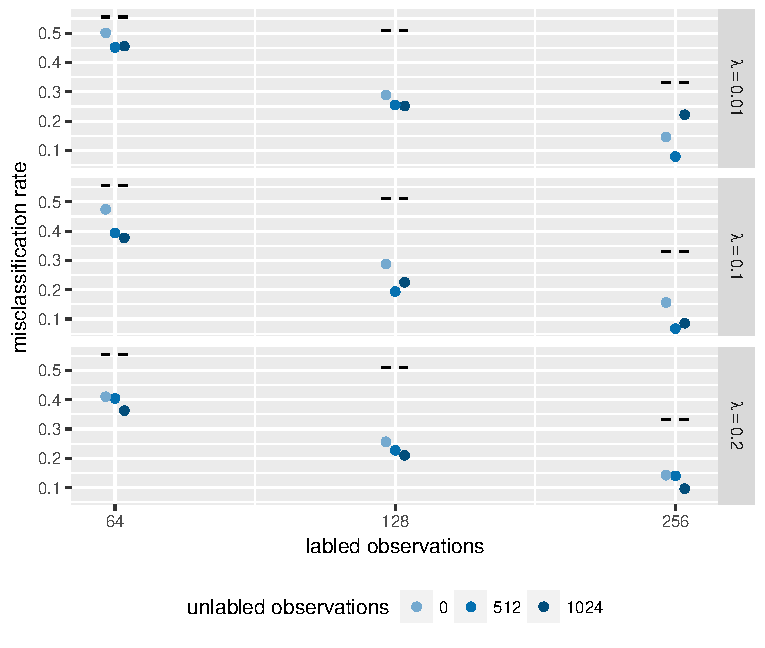
\includegraphics[scale=1]{semi-bytenet/synthetic-digits-grid.pdf}
    \caption{Shows the Semi-Supervised ByteNet model test performance depending on \textit{labeled dataset size}, \textit{unlabeled dataset size}, and \textit{unlabeled learning factor}.}
     \label{fig:result:semi-bytenet:missrate}
\end{figure}

\begin{figure}[h]
    \centering
    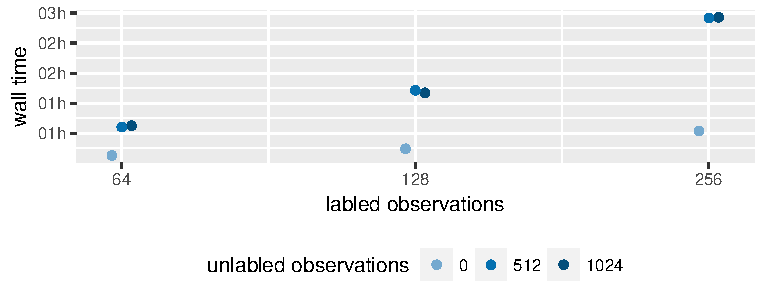
\includegraphics[scale=1]{semi-bytenet/synthetic-digits-grid-time.pdf}
    \caption{Shows the time spend running 300 epochs over the bilingual training dataset. The unlabeled learning rate is aggregated out (mean) since this has no theoretical nor practical performance impact.}
    \label{fig:result:semi-bytenet:time}
\end{figure}

In figure \ref{fig:result:semi-bytenet:time} the performance penalty for using unlabeled observations is very apparent. However, it is not as bad as one would theoretically expect. By using a beam size of 5 sequences, one would expect the training to run 5 times slower, but in practice, it is actually closer to 3. The computational performance is also independent of the unlabeled observations (as long as some are used), this is expected as the number of mini-batches used over 300 epochs only depends on the number of labeled observations.

The good performance can perhaps be explained by how well ByteNet parallelizes over the sequence length. While beam search does prevent this, a computational trick was used to allow some parallelization. By first performing the beam search on the ``text to digit'' translator and reapplying the ``text to digit'' translator (as well as the ``digits to text'' translator) the backward pass on the ``text to digit'' translator could be calculated in parallel. The forward and backward pass on the ``digits to text'' translator can also run in parallel, but this will also be the case for ByteNet. Another contributing factor to the performance is the small dimensionality of the ByteNet models used in the experiment, this likely means that the GPU has plenty of computational resources to run both the supervised and unsupervised part in parallel.

Figure \ref{fig:result:semi-bytenet:missrate} shows similar results to those in the original article, that article the research team found some improvement by using unlabeled observations, but nothing outstanding. This may sound like a disappointment, but in general, it is very hard to improve translation models dramatically. The fact that any translation model can likely be improved by using monolingual (unlabeled) data is actually very encouraging.

A significant difference between this experiment using the synthetic digits dataset and an experiment running on a proper natural language translation dataset is that the digits dataset has no variation in its output given the input. This means that ``one'' will always correspond to one, while in natural languages ``bitten'' in German can be understood as both a ``request'' and as an ''invite'' in English. This means that for a correct translation the unsupervised marginalization will approximately reduce to a marginalization over just one value, which is not very powerful. On the other hand for bad translations which is particularly common during the initial training, having a board beam in the beam search will definitely contribute to the model performance, though the multiple predicted translations in the marginalization. Indeed, if this was not the case it would be very hard to explain the performance improvements. \todo{Not super happy about this part.}

Finally, it is surprising that there is no difference between using 512 or 1024 unlabeled observations, or perhaps even a slight performance penalty for using 1024 unlabeled observations. A reasonable explanation is that using 512 observations covers the vast majority of the variation in the problem, adding the final 1024 observations thus doesn't add much. Furthermore, no insurance was made to prevent duplicate observations (observations was independently sampled). Given that there are only $10^3 + 10^2 = 1100$ different observations, it is very likely that many of the observation are duplicates, this is similar to the birthday probability paradox.

\clearpage

%!TEX root = ../Thesis.tex
\chapter{Conclusion}

Neural machine translation is a difficult and fast moving field. Over the 6 months this thesis has been carried out, several papers with new translation models have published. Each model shows a new state-of-the-part performance over the previous model on the WMT translation task \cite{bytenet, attention-is-all-you-need, tensor2tensor}. These models are created by Google, Microsoft, Facebook, etc., who have both computational resources and man-power to implement and experiment with a huge number of models. The goal and expectation of this thesis is thus not compete with these models, but rather explore a new direction for neural machine translation, by using additional monolingural (unlabeled) data. However, to do this a fast and decent translation model is required, thus much effort have been put into the supervised model.

\paragraph{ByteNet} The ByteNet model was able to learn both the synthetic digits problem and memorize the WMT NewsTest dataset, this confirms the implementation and capabilities of the ByteNet model. For the real problem where the Europarl v7 dataset is used, ByteNet managed to archive a BLEU score of $7.44$ and produce reasonable good translations. This is far from state-of-the-art or just a phase-based (PBMT) baseline model, however given the limited resources the results are rather good.

The original ByteNet paper including the latest revision, did not disclose how much time was spent training or how many resources that were used. From a scientific point of view this is rather inadequate, especially because they created the model from a computational performance perspective. A recent blog-post from Google published in June 2017, compares the different translation models and shows that ByteNet is actually one of the most computationally expensive models \cite{tensor2tensor}.

It is possible that if the oscillation issues were solved, if TensorFlow improving the execution speed with the XLA just-in-time (JIT) compiler \cite{google-xla}, and if CuDNN supported dilated convolution and normalization, that ByteNet could run in reasonable time. However, it will likely take at least a year before TensorFlow and CuDNN are at this state.

\paragraph{Simplified ByteNet} Because ByteNet takes too much time to train, a simplified version of ByteNet was created. Thus has 1/3 the layers and 5/9 the weight, while still maintaining the founding principals behind ByteNet and maintains the dimensional bottleneck. This was done by reducing the embedding dimensionality and removing the dimensional compression and decompression layers.

On the validation problems this performed identically or better compared to the normal ByteNet model. However, when trained on the Europarl v7 dataset the model showed severe overfitting and achieves a test BLEU score of only $0.55$. This indicates that the compression and decompression layers are somehow essential regularization components. In terms of time spend training, the simplified ByteNet model is only 20\% faster and converges correspondingly slower. Profiling the simplified ByteNet model, did unfortunately not reveal why the model is only 20\% faster, but did reveal that normalization is the primary bottleneck in terms of time spent.

The results indicates that simplifying ByteNet is not a direction worth exploring further, at least not for natural language translation. The approach might be valid for simpler problems, but for these problems there are likely completely different model architectures that are better suited.

\paragraph{SELU ByteNet} Identifying that normalization is the primary computational bottleneck, suggests that if these layers can somehow be removed the ByteNet model should perform significantly better. Training a non-normalized ByteNet model on even simple tasks converges very slowly. Recently a paper showed that a special activation called SELU (Self-normalizing Exponential Linear Unit) can be used as a replacement for the typical ReLU and normalization combination. By using the SELU activation as a replacement for ReLU and normalization, the ByteNet model model convergences on the simple tasks.

On the Europarl v7 dataset the SELU ByteNet model does not converge. This appears to be caused by exploding gradients. Such issues could be solved by gradient clipping. However, the purpose of SELU is precisely to prevent exploding and vanishing gradients issues, thus gradient clipping is likely not a good strategy.

In terms of computational performance the SELU ByteNet is much faster than both the normal ByteNet model and the simplified ByteNet model. On the Eurparl v7 problem the SELU ByteNet model runs 13 epochs in 18 hours, the normal ByteNet model uses 4 days on the same number of epochs. Profiling reveal that the time is primarily spent in the SELU activation function. This validates the known issue, where TensorFlow spends an unreasonably amount of time running simple element-wise operations \cite{google-xla}.

From a computational perspective, SELU ByteNet is promising, however as is, it is not suitable for learning translation on the Eurparl v7 dataset. If SELU ByteNet could be made to work, ByteNet would be a serious contender to other models in terms of computation time.

\paragraph{Semi-Supervised ByteNet} Without a suitable fast translation model, it is not feasible to run the semi-supervised ByteNet model on the Europarl v7 dataset. This is because the semi-supervised model depends on two translation models, each running on translations produced by a BeamSearch algorithm. Thus, one should expect the semi-supervised model to take 10 times longer to train. 

With the the computational demands of ByteNet in mind, the semi-supervised ByteNet model was used on a synthetic problem translating spelled-out digits to digit symbols. For example, ``one zero four'' is translated to ``104''. On this problem the semi-supervised ByteNet model showed improvement over both the supervised ByteNet model and an attention-based baseline model.

This validates the results from the original paper \cite{semi-supervised}, where the BELU score could be improved by $3.5$ to $1.5$. While such an improvement doesn't completely solve all issues, when training on language-pairs where the bilingual dataset is small, it could be an important component when the bilingual data isn't plentiful but the monolingural data is.

% While the semi-supervised model is not mathematically interesting, it is a pragmatic approach that works well with models that have fast/linear-time inference, such as ByteNet. However the ByteNet model is too slow for it to be relevant.

\paragraph{Future Works} With the resent results published by Google, showing that ByteNet is actually one of the slowest machine translation models \cite{tensor2tensor}, ByteNet is not a likely model for neural machine translation, and even less likely as a semi-supervised model. It is possible that the SELU ByteNet model could be tuned to work, in which case it might be compatible model. More time should be spent exporing the underlying cause and possible solutions to the exploding gradient issues in SELU ByteNet.

Recently a new paper showed that attention can be used instead of bi-directional RNN layers or hieratical-dilated-convolution. Using this approach they created a neural machine translation model that achieves a new state-of-the-art BLEU score on en-de translation. The model is also faster than many previous models, as it is shares many of the founding principals of ByteNet. That is, resolution persistent encoding, parallelization over the sequences, and training in linear time, are essential properties \cite{attention-is-all-you-need}.

Such a translation model is close to ideal, to be used in combination with the semi-supervised approach. Although, because the model is based on attention inference can't be done in linear time, unlike ByteNet, which may be essential for computing the unsupervised part of the loss-function. That being said, it is only the forward pass of one of the translation models that will run in quadratic time. The both backward passes and the other translation model will run in linear-time.

A different approach for making the semi-supervised model converge within reasonable time, is to initialize the weights with the learned weights from the two translation models it uses, where the translation models are pre-trained on a bilingual dataset. This would work as a pseudo-transfer learning, ``pseudo'' because the application domain is the same and it is the same models that are used. While this may improve convergence for a reasonable fast translation model, ByteNet is still too slow to be fully trained on just a single bilingual dataset.

Finally, one could look at a completely different approach for semi-supervised machine translation. In image processing adversarial networks have been successfully used to ``translate'' between for example a zebra and a horse, without paired training data \cite{gan-image-translation}. A similar approach could perhaps be used in the field of natural language translation. However, the current state of adversarial networks for natural languages is still far behind compared to other applications \cite{gan-on-nlp}.

\appendix
%!TEX root = ../Thesis.tex
\chapter{Notation}


\begin{table}[H]
\centering
\begin{tabular}{r p{10cm}}
	symbol & meaning \\ \hline
	% Nework
	$z$ & The activation input, calculated as a weighted sum over the input. \\
	$a$ & The activation output, $a = \theta(z)$. \\
	$\theta$ & The non-linear activation function. \\
	$H$ & The amount of units in the layer. \\
	$h$ & The index of a units in the layer. \\
	$K$ & The amount of classes calculated in the softmax, $K = H_{L+1}$. \\ 
	$\ell$ & The layer index. \\
	$L$ & The amount of hidden layers. Including the softmax output layer there are $L+1$ layers. \\
	$t$ & A target value. If used in a superscript it is the sequence index. \\
	$w$ & A weight used in a neural neural network. \\
	$x$ & The input to the neural network, $x = z_{h_0}$. \\
	$y$ & The softmax output. \\
	
	% Optimization
	$\mathcal{L}$ & The loss function (should always be minimized). \\
	$\delta$ & Bookkeeping value used in backward propagation. \\
	$\alpha$ & Learning rate used in the Adam Optimization algorithm. \\
	
	% Normalization
	$\gamma$ & Scale parameter in normalization. \\
	$\beta$ & Bias parameter in normalization. \\

    % Dilated convolution
	$d$ & The dimensionality of the vector representation. \\
    $*$ & The convolution operator. \\
    $\otimes$ & The Kronecker product. \\
	$k$ & The kernel width in a 1d-convolution. \\
	$r$ & The dilation rate used in dilated convolution. \\
    
	% BeamSearch
	$b$ & The beam size used in the BeamSearch algorithm.
\end{tabular}
\caption*{\textbf{Table A.1: } Meaning of commonly used symbols.}
\end{table}

\begin{figure}[H]
	\vspace{-0.1cm}
	\centering
	\includegraphics[scale=1]{appendices/notation}
	\caption*{\textbf{Figure A.1: } A two-level subscript is used for the neuron index.}
\end{figure}

\chapter{Backward Pass}

\section{Softmax}
\label{appendix:backward-pass:softmax}

The forward pass for the softmax and the cross entropy loss is given by:

\begin{equationbox}[H]
\begin{equation*}
\begin{aligned}
y_k &= \frac{\exp(z_k)}{\sum_{k'=1}^K \exp(z_{k'})}, && \text{ where: } z_k=z_{h_{L+1}}, K = H_{L + 1} \\
\mathcal{L} &= - \sum_{k=1}^K t_k \ln(y_k)
\end{aligned}
\end{equation*}
\caption{Forward equations Cross Entropy loss with Softmax input.}
\end{equationbox}

The last delta ($\delta_{h_{L+1}}$) is what should be derived:
\begin{equation}
\delta_{h_{L + 1}} = \delta_k = \frac{\partial \mathcal{L}}{\partial z_k} = \sum_{k'=1}^K \frac{\partial \mathcal{L}}{\partial y_{k'}} \frac{\partial y_{k'}}{\partial z_k} = y_k - t_k
\label{appendix:backprop:softmax:bprop-delta-last}
\end{equation}

The first derivative $\frac{\partial \mathcal{L}}{\partial y_{k'}}$ is derived from the cross entropy equation:
\begin{equation}
\frac{\partial \mathcal{L}}{\partial y_{k'}} = \frac{\partial}{\partial y_{k'}} \left(- \sum_{k''=1}^K t_{k''} \ln(y_{k''})\right) = -\frac{t_{k'}}{y_{k'}}
\label{appendix:backprop:softmax:bprop-Ldy}
\end{equation}

The other derivative $\frac{\partial y_{k'}}{\partial z_k}$ can be derived from the softmax function:
\begin{equation}
\begin{aligned}
\frac{\partial y_{k'}}{\partial z_k}
&= \frac{\partial}{\partial z_k} \frac{\exp(z_{k'})}{\sum_{k''=1}^K \exp(z_{k''})} \\
&= \frac{\frac{\partial}{\partial z_k} \exp(z_{k'})}{\sum_{k''=1}^K \exp(z_{k''})}
- \frac{\exp(z_{k'}) \frac{\partial}{\partial z_k} \sum_{k''=1}^K \exp(z_{k''})}{\left(\sum_{k''=1}^K \exp(z_{k''})\right)^2} \\
&= \frac{\frac{\partial}{\partial z_k} \exp(z_{k'})}{\sum_{k''=1}^K \exp(z_{k''})}
- \frac{\exp(z_{k'})}{\sum_{k''=1}^K \exp(z_{k''})} \frac{\frac{\partial}{\partial z_k} \sum_{k''=1}^K \exp(z_{k''})}{\sum_{k''=1}^K \exp(z_{k''})}
\end{aligned}
\end{equation}

Because of the difference in index, the first term is only not zero when $k = k'$, in which case $y_k$ is the derivative. It thus becomes useful to define:
\begin{equation}
\delta_{i,j} = \begin{cases}1& \text{when } i = j \\ 0 & \text{otherwise}\end{cases}
\end{equation}

Similarly in the second term $\frac{\partial}{\partial z_k} \exp(z_{k''})$ is zero except in the case where $k = k''$:
\begin{equation}
\frac{\partial y_{k'}}{\partial a_k} = \delta_{k, k'} y_k - y_{k'} y_k
\label{appendix:backprop:softmax:bprop-yda}
\end{equation}

The result from \eqref{appendix:backprop:softmax:bprop-Ldy} and \eqref{appendix:backprop:softmax:bprop-yda} is then combined into \eqref{appendix:backprop:softmax:bprop-delta-last}:
\begin{equation}
\begin{aligned}
\delta_{h_{L + 1}} = \delta_k &= \sum_{k'=1}^K -\frac{t_{k'}}{y_{k'}} \left( \delta_{k, k'} y_k - y_{k'} y_k \right) = \sum_{k'=1}^K -\frac{t_{k'}}{y_{k'}} \delta_{k, k'} y_k + \sum_{k'=1}^K \frac{t_{k'}}{y_{k'}} y_{k'} y_k \\
&= -\frac{t_k}{y_k} y_k + y_k \sum_{k'=1}^K t_{k'} = -t_k + y_k = y_k - t_k
\end{aligned}
\label{appendix:backprop:softmax:bprop-deltaKfinal}
\end{equation}

To get $\sum_{k'=1}^K t_{k'} = 1$ it's used that $\{ t_{k'} \}_{k'=1}^K$ is the target distribution and thus must sum to 1.

\section{Dilated Convolution}
\label{appendix:backward-pass:dilated-convolution}

\begin{equationbox}[H]
\begin{equation*}
\begin{aligned}
z_{h_\ell}(t) &= (a_{\ell-1} *_r w_{:, h_\ell})(t) = \sum_{h_{\ell-1}}^{H_{\ell-1}} \sum_{i} a_{h_{\ell-1}}(t + r\,i) w_{h_{\ell-1}, h_\ell}(i) \\
a_{h_\ell}(t) &= \theta(z_{h_\ell}(t))
\end{aligned}
\end{equation*}
\caption{Forward equations for Dilated Convolution.}
\end{equationbox}

For deriving the backward pass the padding will be ignored, this is not a big issue as the input image $a_{\ell-1}$ can easily be extended. It also turns out that the final derivative makes the generalization quite intuitive.

For the backward pass we just which to derive:
\begin{equation}
\frac{\partial \mathcal{L}}{\partial w_{h_{\ell-1},h_\ell}(i)}
\end{equation}

The weight $w_{h_{\ell-1},h_\ell}(i)$ affects all time steps, thus the chain rule yields:
\begin{equation}
\begin{aligned}
\frac{\partial \mathcal{L}}{\partial w_{h_{\ell-1},h_\ell}(i)} &= \sum_{t} \frac{\partial \mathcal{L}}{\partial z_{h_\ell}(t)} \frac{z_{h_\ell}(t)}{\partial w_{h_{\ell-1},h_\ell}(i)} \\
&= \sum_{t} \delta_{h_\ell}(t) a_{h_{\ell-1}}(t + r\,i)
\end{aligned}
\end{equation}
\todo[inline]{somehow this can be rewritten to a convolution: $(\delta_{h_\ell} * rot(a_{h_{\ell-1}}))(i)$, see \url{https://grzegorzgwardys.wordpress.com/2016/04/22/8/}}

Here $\delta_{h_\ell}(t)$ is defined as:
\begin{equation}
\delta_{h_\ell}(t) \defeq \frac{\partial \mathcal{L}}{\partial z_{h_\ell}}(t)
\end{equation}

To calculate $\delta_{h_\ell}(t)$ the chain rule is used again, the first step is easy:
\begin{equation}
\delta_{h_\ell}(t) = \frac{\partial \mathcal{L}}{\partial z_{h_\ell}(t)} = \frac{\partial \mathcal{L}}{\partial a_{h_\ell}(t)} \frac{\partial a_{h_\ell}(t)}{\partial z_{h_\ell}(t)} = \theta'(z_{h_\ell}(t)) \frac{\partial \mathcal{L}}{\partial a_{h_\ell}(t)}
\end{equation}

The next steps are more complicated, $a_{h_\ell}(t)$ affects $z_{h_{\ell+1}}(t')$ for all channels in the next layer, and all times $t'$ that are within the kernel width of $t$.
\begin{equation*}
\delta_{h_\ell}(t) = \theta'(z_{h_\ell}(t)) \frac{\partial \mathcal{L}}{\partial a_{h_\ell}(t)} = \theta'(z_{h_\ell}(t)) \sum_{h_{\ell+1}=1}^{H_{\ell+1}} \sum_{i} \frac{\partial \mathcal{L}}{\partial z_{h_{\ell+1}}(t + r\, i)} \frac{\partial z_{h_{\ell+1}}(t + r\, i)}{\partial a_{h_\ell}(t)}
\end{equation*}

To derive $\frac{\partial z_{h_{\ell+1}}(t + r\, i)}{\partial a_{h_\ell}(t)}$ it helps to write out $z_{h_{\ell+1}}(t + r\, i)$.
\begin{equation}
z_{h_{\ell+1}}(t + r\, i) = (a_{\ell} * w_{:,h_\ell})(t + r\, i) = \sum_{h_\ell}^{H_\ell} \sum_{i'} a_{h_\ell}(t + r\, i + r\, i') w_{h_\ell, h_{\ell+1}}(i')
\end{equation}
From this one can observe that $t + r\, i + r\, i' = t$ only occurs when $i' = -i$, thus the $\delta_{h_\ell}(t)$ derivative becomes:
\begin{equation}
\begin{aligned}
\delta_{h_\ell}(t) &= \theta'(z_{h_\ell}(t)) \sum_{h_{\ell+1}=1}^{H_{\ell+1}} \sum_{i} \frac{\partial \mathcal{L}}{\partial z_{h_{\ell+1}}(t + r\, i)} w_{h_\ell, h_{\ell+1}}(-i) \\
&= \theta'(z_{h_\ell}(t)) \sum_{h_{\ell+1}=1}^{H_{\ell+1}} \sum_{i} \delta_{h_{\ell+1}}(t + r\, i) w_{h_\ell, h_{\ell+1}}(-i)
\end{aligned}
\end{equation}

This is actually a dilated convolution, just where the weight is flipped (rotated).
\begin{equation}
\delta_{h_\ell}(t) = \theta'(z_{h_\ell}(t)) (\delta_{\ell + 1} *_r \mathrm{rot}(w_{:, h_{\ell + 1}}))(t)
\end{equation}

This is the derivative for the dilated convolution. Because the derivative is a convolution itself, it naturally generalizes to any padding implementation. 

\clearpage
\section{Batch Normalization}
\label{appendix:backward-pass:batch-norm}

To derive the backward pass for batch normalization it helps to setup equations for $\mathbb{E}[z_{h_\ell}]$ and $\textsc{Var}[z_{h_\ell}]$. To do this we need to reintroduce the observation index this time it will be denoted with the superscript $(i)$. Similarly, the mini-batch will be denoted with $\mathcal{B}$. With these changes the the full forward pass can be written as:
\begin{equationbox}[H]
Activation:
\begin{equation*}
\begin{aligned}
z_{h_\ell}^{(i)} &= \sum_{h_{\ell-1}}^{H_{\ell-1}} w_{h_{\ell-1},h_\ell} a_{h_\ell-1}^{(i)} \\
\hat{z}_{h_\ell}^{(i)} &= \gamma_{h_\ell} \frac{z_{h_\ell}^{(i)} - \mu_{h_\ell}^{\mathcal{B}}}{\sqrt{\sigma_{h_\ell}^{2,\mathcal{B}} + \epsilon}} + \beta_{h_\ell} \\
a_{h_\ell}^{(i)} &= \theta\left(\hat{z}_{h_\ell}^{(i)}\right)
\end{aligned}
\end{equation*}
Statistics:
\begin{equation*}
\begin{aligned}
\mu_{h_\ell}^{\mathcal{B}} &= \frac{1}{n} \sum_{i=1}^n z_{h_\ell}^{(i)} \\
\sigma_{h_\ell}^{2, \mathcal{B}} &= \frac{1}{n} \sum_{i=1}^n (z_{h_\ell}^{(i)} - \mu_{h_\ell}^{\mathcal{B}})^2
\end{aligned}
\end{equation*}
\caption{Forward equations for Batch Normalization.}
\end{equationbox}

Now that the forward pass is stated explicitly, the backward pass can be derived. For the backward pass we which to derive:
\begin{equation}
\frac{\partial \mathcal{L}}{\partial w_{h_{\ell-1},h_\ell}},\quad \frac{\partial \mathcal{L}}{\partial \gamma_{h_\ell}},\quad \frac{\partial \mathcal{L}}{\partial \beta_{h_\ell}}
\end{equation}

The gradient with respect to the weight $w_{h_{\ell-1},h_\ell}$ hasn't changed:
\begin{equation}
\frac{\partial \mathcal{L}}{\partial w_{h_{\ell-1},h_\ell}} = \sum_{i=1}^n \frac{\partial \mathcal{L}}{\partial z_{h_\ell}^{(i)}} \frac{\partial z_{h_\ell}^{(i)}}{\partial w_{h_{\ell-1},h_\ell}} =\sum_{i=1}^n \delta_{h_\ell}^{(i)} a_{h_{\ell-1}}^{(i)}
\end{equation}
Note that without batch normalization the sum over the observations does not directly appear in the gradients, but this is only because the observation index $i$ is omitted. In reality, it sums the gradients for each observation in the mini-batch.

The $\delta_{h_\ell}$ however has changed quite significantly:
\begin{equation}
\begin{aligned}
\delta_{h_\ell}^{(i)} = \frac{\partial \mathcal{L}}{\partial z_{h_\ell}^{(i)}} &= \frac{\partial \mathcal{L}}{\partial \hat{z}_{h_\ell}^{(i)}} \frac{\partial \hat{z}_{h_\ell}^{(i)}}{\partial z_{h_\ell}^{(i)}} + \frac{\partial \mathcal{L}}{\partial \sigma_{h_\ell}^{2,\mathcal{B}}} \frac{\partial \sigma_{h_\ell}^{2,\mathcal{B}}}{\partial z_{h_\ell}^{(i)}} + \frac{\partial \mathcal{L}}{\partial \mu_{h_\ell}^{\mathcal{B}}} \frac{\partial \mu_{h_\ell}^{\mathcal{B}}}{\partial z_{h_\ell}^{(i)}} \\
&= \frac{\partial \mathcal{L}}{\partial \hat{z}_{h_\ell}^{(i)}} \frac{\gamma_{h_\ell}}{\sqrt{\sigma_{h_\ell}^{2, \mathcal{B}} + \epsilon}} + \frac{\partial \mathcal{L}}{\partial \sigma_{h_\ell}^{2,\mathcal{B}}} \frac{2}{n}\left(z_{h_\ell}^{(i)} - \mu_{h_\ell}^{\mathcal{B}}\right) + \frac{\partial \mathcal{L}}{\partial \mu_{h_\ell}^{\mathcal{B}}} \frac{1}{n}
\end{aligned}
\label{eq:appendix:batch-norm:delta}
\end{equation}

From \eqref{eq:appendix:batch-norm:delta} the following derivatives also needs to be derived:
\begin{equation}
\frac{\partial \mathcal{L}}{\partial \hat{z}_{h_\ell}^{(i)}}, \quad \frac{\partial \mathcal{L}}{\partial \sigma_{h_\ell}^{2,\mathcal{B}}}, \quad \frac{\partial \mathcal{L}}{\partial \mu_{h_\ell}^{\mathcal{B}}}
\end{equation}

As with everything else, this is done by using the chain rule:
\begin{equation}
\frac{\partial \mathcal{L}}{\partial \hat{z}_{h_\ell}^{(i)}} = \frac{\partial \mathcal{L}}{\partial a_{h_\ell}^{(i)}} \frac{\partial a_{h_\ell}^{(i)}}{\partial \hat{z}_{h_\ell}^{(i)}} = \theta'(\hat{z}_{h_\ell}^{(i)}) \frac{\partial\mathcal{L}}{\partial a_{h_\ell}^{(i)}} = \theta'(\hat{z}_{h_\ell}^{(i)}) \sum_{h_{\ell+1}}^{H_{\ell+1}} \delta_{h_{\ell+1}}^{(i)} w_{h_\ell, h_{\ell+1}}
\end{equation}
\begin{equation}
\frac{\partial \mathcal{L}}{\partial \sigma_{h_\ell}^{2,\mathcal{B}}} = \sum_{i=1}^n \frac{\partial \mathcal{L}}{\partial \hat{z}_{h_\ell}^{(i)}} \frac{\partial \hat{z}_{h\ell}^{(i)}}{\partial \sigma_{h_\ell}^{2, \mathcal{B}}} = \sum_{i=1}^n \frac{\partial \mathcal{L}}{\partial \hat{z}_{h_\ell}^{(i)}} \gamma_{h_\ell} \left(z_{h_\ell}^{(i)} - \mu_{h_\ell}^{\mathcal{B}}\right) \left(-\frac{1}{2}\right) \left(\sigma_{h_\ell}^{\mathcal{B}} + \epsilon\right)^{-\frac{2}{3}}
\end{equation}
\begin{equation}
\begin{aligned}
\frac{\partial \mathcal{L}}{\partial \mu_{h_\ell}^{\mathcal{B}}} &= \sum_{i=1}^n \frac{\partial \mathcal{L}}{\partial \hat{z}_{h_\ell}^{(i)}} \frac{\partial \hat{z}_{h_\ell}^{(i)}}{\mu_{h_\ell}^{\mathcal{B}}} + \frac{\partial \mathcal{L}}{\partial \sigma_{h_\ell}^{2, \mathcal{B}}} \frac{\partial \sigma_{h_\ell}^{2, \mathcal{B}}}{\mu_{h_\ell}^{\mathcal{B}}} \\
&= \sum_{i=1}^n \frac{\partial \mathcal{L}}{\partial \hat{z}_{h_\ell}^{(i)}} \left(- \frac{1}{\sqrt{\sigma_{h_\ell}^{2, \mathcal{B}} + \epsilon}}\right) + \frac{\partial \mathcal{L}}{\partial \sigma_{h_\ell}^{2, \mathcal{B}}} \frac{1}{n} \sum_{i=1}^n -2 \left(z_{h_\ell}^{(i)} - \mu_{h_\ell}^{\mathcal{B}}\right)
\end{aligned}
\end{equation}

Finally, the gradient with respect to $\gamma_{h_\ell}$ and $\beta_{h_\ell}$ can be derived:
\begin{equation}
\frac{\partial \mathcal{L}}{\partial \gamma_{h_\ell}} = \sum_{i=1}^n \frac{\partial \mathcal{L}}{\partial \hat{z}_{h_\ell}^{(i)}} \frac{\partial \hat{z}_{h_\ell}^{(i)}}{\partial \gamma_{h_\ell}} = \sum_{i=1}^n \frac{\partial \mathcal{L}}{\partial \hat{z}_{h_\ell}^{(i)}} \left(\frac{z_{h_\ell}^{(i)} - \mu_{h_\ell}^{\mathcal{B}}}{\sqrt{\sigma_{h_\ell}^{2, \mathcal{B}} + \epsilon}} \right)
\end{equation}
\begin{equation}
\frac{\partial \mathcal{L}}{\partial \beta_{h_\ell}} = \sum_{i=1}^n \frac{\partial \mathcal{L}}{\partial \hat{z}_{h_\ell}^{(i)}} \frac{\partial \hat{z}_{h_\ell}^{(i)}}{\partial \beta_{h_\ell}} = \sum_{i=1}^n \frac{\partial \mathcal{L}}{\partial \hat{z}_{h_\ell}^{(i)}}
\end{equation}

These only depend on $\frac{\partial \mathcal{L}}{\partial \hat{z}_{h_\ell}^{(i)}}$ which has already been derived.

\clearpage
\section{Layer Normalization}

Let's repeat the forward pass:
\begin{equationbox}[H]
\begin{equation*}
\begin{aligned}
z_{h_\ell} &= \sum_{h_{\ell-1}}^{H_{\ell-1}} w_{h_{\ell-1},h_\ell} a_{h_\ell-1} \\
\hat{z}_{h_\ell} &= \gamma_{h_\ell} \frac{z_{h_\ell} - \mu_{\ell}}{\sqrt{\sigma_{\ell}^2 + \epsilon}} + \beta_{h_\ell} \\
a_{h_\ell} &= \theta\left(\hat{z}_{h_\ell}\right)
\end{aligned}
\end{equation*}
Statistics:
\begin{equation*}
\begin{aligned}
\mu_{\ell} &= \frac{1}{H_\ell} \sum_{h_\ell}^{H_\ell} z_{h_\ell} \\
\sigma_{\ell}^2 &= \frac{1}{H_\ell} \sum_{h_\ell}^{H_\ell} (z_{h_\ell} - \mu_{\ell})^2
\end{aligned}
\end{equation*}
\caption{Forward equations for Layer Normalization.}
\end{equationbox}

For the backward pass we which to derive:
\begin{equation}
\frac{\partial \mathcal{L}}{\partial w_{h_{\ell-1},h_\ell}},\quad \frac{\partial \mathcal{L}}{\partial \gamma_{h_\ell}},\quad \frac{\partial \mathcal{L}}{\partial \beta_{h_\ell}}
\end{equation}

The gradient with respect to the weight $w_{h_{\ell-1},h_\ell}$ is the same:

\begin{equation}
\frac{\partial \mathcal{L}}{\partial w_{h_{\ell-1},h_\ell}} = \frac{\partial \mathcal{L}}{\partial z_{h_\ell}} \frac{\partial z_{h_\ell}}{\partial w_{h_{\ell-1},h_\ell}} = \delta_{h_\ell} a_{h_{\ell-1}}
\end{equation}

Like in Batch Normalization $\delta_{h_\ell}$ has changed quite significantly:

\begin{equation}
\begin{aligned}
\delta_{h_\ell} = \frac{\partial \mathcal{L}}{\partial z_{h_\ell}} &= \frac{\partial \mathcal{L}}{\partial \hat{z}_{h_\ell}} \frac{\partial \hat{z}_{h_\ell}}{\partial z_{h_\ell}} + \frac{\partial \mathcal{L}}{\partial \sigma_{\ell}^2} \frac{\partial \sigma_{\ell}^2}{\partial z_{h_\ell}} + \frac{\partial \mathcal{L}}{\partial \mu_{\ell}} \frac{\partial \mu_{\ell}}{\partial z_{h_\ell}} \\
&= \frac{\partial \mathcal{L}}{\partial \hat{z}_{h_\ell}} \frac{\gamma_{h_\ell}}{\sqrt{\sigma_{\ell}^2 + \epsilon}} + \frac{\partial \mathcal{L}}{\partial \sigma_{\ell}^2} \frac{2}{H_\ell}\left(z_{h_\ell} - \mu_{\ell}\right) + \frac{\partial \mathcal{L}}{\partial \mu_{\ell}} \frac{1}{H_\ell}
\end{aligned}
\label{eq:appendix:layer-norm:delta}
\end{equation}

From \eqref{eq:appendix:layer-norm:delta} the following derivatives also needs to be derived:
\begin{equation}
\frac{\partial \mathcal{L}}{\partial \hat{z}_{h_\ell}}, \quad \frac{\partial \mathcal{L}}{\partial \sigma_{\ell}^2}, \quad \frac{\partial \mathcal{L}}{\partial \mu_{\ell}}
\end{equation}

As with everything else this is done by using the chain rule:
\begin{equation}
\frac{\partial \mathcal{L}}{\partial \hat{z}_{h_\ell}} = \frac{\partial \mathcal{L}}{\partial a_{h_\ell}} \frac{\partial a_{h_\ell}}{\partial \hat{z}_{h_\ell}} = \theta'(\hat{z}_{h_\ell}) \frac{\partial \mathcal{L}}{\partial a_{h_\ell}} = \theta'(\hat{z}_{h_\ell}) \sum_{h_{\ell+1}}^{H_{\ell+1}} \delta_{h_{\ell+1}} w_{h_\ell, h_{\ell+1}}
\end{equation}

\begin{equation}
\frac{\partial \mathcal{L}}{\partial \sigma^2_\ell} = \sum_{h_\ell}^{H_\ell} \frac{\partial \mathcal{L}}{\partial \hat{z}_{h_\ell}} \frac{\partial \hat{z}_{h_\ell}}{\partial \sigma_\ell^2} = \sum_{h_\ell}^{H_\ell} \frac{\partial \mathcal{L}}{\partial \hat{z}_{h_\ell}} \gamma_{h_\ell} (z_{h_\ell} - \mu_\ell) \left(- \frac{1}{2}\right) \left(\sigma_\ell^2 + \epsilon\right)^{-\frac{2}{3}}
\end{equation}

\begin{equation}
\begin{aligned}
\frac{\partial \mathcal{L}}{\partial \mu_\ell} &= \sum_{h_\ell}^{H_\ell} \frac{\partial \mathcal{L}}{\partial \hat{z}_{h_\ell}} \frac{\partial \hat{z}_{h_\ell}}{\partial \mu_\ell} + \frac{\partial \mathcal{L}}{\partial \sigma_{\ell}^2} \frac{\partial \sigma_\ell^2}{\partial \mu_\ell} \\
&= \sum_{h_\ell}^{H_\ell} \frac{\partial \mathcal{L}}{\partial \hat{z}_{h_\ell}} \left(- \frac{1}{\sqrt{\sigma_\ell^2 + \epsilon}}\right) + \frac{\partial \mathcal{L}}{\partial \sigma_{\ell}^2} \frac{1}{H_\ell} \sum_{h_\ell}^{H_\ell} -2 \left(z_{h_\ell} - \mu_\ell\right)
\end{aligned}
\end{equation}

Finally, the gradient with respect to $\gamma_{h_\ell}$ and $\beta_{h_\ell}$ can be derived:

\begin{equation}
\frac{\partial \mathcal{L}}{\partial \gamma_{h_\ell}} = \frac{\partial \mathcal{L}}{\partial \hat{z}_{h_\ell}} \frac{\partial \hat{z}_{h_\ell}}{\partial \gamma_{h_\ell}} = \frac{\partial \mathcal{L}}{\partial \hat{z}_{h_\ell}} \left(\frac{z_{h_\ell} - \mu_\ell}{\sqrt{\sigma_\ell^2 + \epsilon}}\right)
\end{equation}

\begin{equation}
\frac{\partial \mathcal{L}}{\partial \beta_{h_\ell}} = \frac{\partial \mathcal{L}}{\partial \hat{z}_{h_\ell}} \frac{\partial \hat{z}_{h_\ell}}{\partial \beta_{h_\ell}} = \frac{\partial \mathcal{L}}{\partial \hat{z}_{h_\ell}}
\end{equation}

These only depend on $\frac{\partial \mathcal{L}}{\partial \hat{z}_{h_\ell}}$ which has already been derived.

\section{Semi-Supervised Marginalization}
\label{appendix:backward-pass:semi-sum}

\begin{equationbox}[H]
\begin{equation*}
\mathcal{L} = -\log(P(\mathbf{y}'|\mathbf{y}, \overrightarrow{\boldsymbol\theta}, \overleftarrow{\boldsymbol\theta}))
\end{equation*}
Monolingual translation model:
\begin{equation*}
P(\mathbf{y}'|\mathbf{y}, \overrightarrow{\boldsymbol\theta}, \overleftarrow{\boldsymbol\theta}) = \sum_{\mathbf{x}} P(\mathbf{y}'|\mathbf{x}, \overrightarrow{\boldsymbol\theta}) P(\mathbf{x}|\mathbf{y}, \overleftarrow{\boldsymbol\theta})
\end{equation*}
\caption{Loss function for the semi-supervised model.}
\end{equationbox}

To optimize the loss the gradient with respect to $\overrightarrow{\boldsymbol\theta}$ is calculated. The gradient with respect to $\overleftarrow{\boldsymbol\theta}$ is also needed, but that is symmetrically similar to the $\overrightarrow{\boldsymbol\theta}$ gradient.
\begin{equation}
\frac{\partial}{\partial \overrightarrow{\boldsymbol\theta}} \mathcal{L} = \frac{\partial}{\partial \overrightarrow{\boldsymbol\theta}} -\log(P(\mathbf{y}'|\mathbf{y}, \overrightarrow{\boldsymbol\theta}, \overleftarrow{\boldsymbol\theta}))
\end{equation}

Start out by differentiating the $\log(\cdot)$ function and insert the expression for $P(\mathbf{y}'|\mathbf{y}, \overrightarrow{\boldsymbol\theta}, \overleftarrow{\boldsymbol\theta})$:
\begin{equation}
\begin{aligned}
\frac{\partial}{\partial \overrightarrow{\boldsymbol\theta}} -\log(P(\mathbf{y}'|\mathbf{y}, \overrightarrow{\boldsymbol\theta}, \overleftarrow{\boldsymbol\theta}))
&= - \frac{\frac{\partial}{\partial \overrightarrow{\boldsymbol\theta}} P(\mathbf{y}'|\mathbf{y}, \overrightarrow{\boldsymbol\theta}, \overleftarrow{\boldsymbol\theta})}{P(\mathbf{y}'|\mathbf{y}, \overrightarrow{\boldsymbol\theta}, \overleftarrow{\boldsymbol\theta})} \\
&= - \frac{\sum_{\mathbf{x}} \frac{\partial}{\partial \overrightarrow{\boldsymbol\theta}} P(\mathbf{y}'|\mathbf{x}, \overrightarrow{\boldsymbol\theta}) P(\mathbf{x}|\mathbf{y}, \overleftarrow{\boldsymbol\theta})}{\sum_{\mathbf{x}} P(\mathbf{y}'|\mathbf{x}, \overrightarrow{\boldsymbol\theta}) P(\mathbf{x}|\mathbf{y}, \overleftarrow{\boldsymbol\theta})}
\end{aligned}
\end{equation}

The identity $\frac{\partial f({\boldsymbol\theta})}{\partial {\boldsymbol\theta}} = f({\boldsymbol\theta}) \frac{\partial \log(f({\boldsymbol\theta}))}{\partial {\boldsymbol\theta}}$ is then applied.
\begin{equation}
\frac{\partial}{\partial \overrightarrow{\boldsymbol\theta}} -\log(P(\mathbf{y}'|\mathbf{y}, \overrightarrow{\boldsymbol\theta}, \overleftarrow{\boldsymbol\theta})) = - \frac{\sum_{\mathbf{x}} P(\mathbf{y}'|\mathbf{x}, \overrightarrow{\boldsymbol\theta}) P(\mathbf{x}|\mathbf{y}, \overleftarrow{\boldsymbol\theta}) \frac{\partial}{\partial \overrightarrow{\boldsymbol\theta}} \log(P(\mathbf{y}'|\mathbf{x}, \overrightarrow{\boldsymbol\theta})) }{\sum_{\mathbf{x}} P(\mathbf{y}'|\mathbf{x}, \overrightarrow{\boldsymbol\theta}) P(\mathbf{x}|\mathbf{y}, \overleftarrow{\boldsymbol\theta})}
\end{equation}

Calculating $\frac{\partial}{\partial \overrightarrow{\boldsymbol\theta}} \log(P(\mathbf{y}'|\mathbf{x}, \overrightarrow{\boldsymbol\theta}))$ is more numerically stable than calculating $\frac{\partial}{\partial \overrightarrow{\boldsymbol\theta}} P(\mathbf{y}'|\mathbf{x}, \overrightarrow{\boldsymbol\theta})$ directly. Furthermore, since $P(\mathbf{y}'|\mathbf{x}, \overrightarrow{\boldsymbol\theta})$ already has to be calculated there is also no loss in performance.

\chapter{Numerical Stability}

\section{The log-softmax function}
\label{appendix:numerical-stability:log-softmax}
% https://github.com/tensorflow/tensorflow/blob/master/tensorflow/core/kernels/softmax_op_functor.h#L73L83

\begin{equationbox}[H]
\begin{equation*}
\mathcal{S}(\mathbf{x})_i = \frac{\mathrm{exp}(x_i)}{\sum_j \mathrm{exp}(x_j)}
\end{equation*}
\caption{The softmax function on input vector $\mathbf{x}$.}
\end{equationbox}

To make the softmax function numerically stable the maximal value of the input vector $\mathbf{x}$ is subtracted, this is denotes as the alternative softmax function $\tilde{\mathcal{S}}(\mathbf{x}) = \mathcal{S}(\mathbf{x} - \mathrm{max}(\mathbf{x}))$.

The alternative softmax function $\tilde{\mathcal{S}}(\mathbf{x})$ is then simplified:
\begin{equation}
\begin{aligned}
\tilde{\mathcal{S}}(\mathbf{x})_i
&= \frac{\mathrm{exp}(x_i - \mathrm{max}(\mathbf{x})))}{\sum_j \mathrm{exp}(x_j - \mathrm{max}(\mathbf{x})))} \\
&= \frac{\mathrm{exp}(x_i)\mathrm{exp}(- \mathrm{max}(\mathbf{x})))}{\sum_j \mathrm{exp}(x_j)\mathrm{exp}(- \mathrm{max}(\mathbf{x})))} \\
&= \frac{\mathrm{exp}(x_i)\mathrm{exp}(- \mathrm{max}(\mathbf{x})))}{\mathrm{exp}(- \mathrm{max}(\mathbf{x}))) \sum_j \mathrm{exp}(x_j)} \\
&= \frac{\mathrm{exp}(x_i)}{\sum_j \mathrm{exp}(x_j)} \\
&= \mathcal{S}(\mathbf{x})_i
\end{aligned}
\label{eq:appendix:numerical:log-softmax:softmax-mmax}
\end{equation}

As seen from \eqref{eq:appendix:numerical:log-softmax:softmax-mmax} the alternative softmax function $\tilde{\mathcal{S}}(\mathbf{x})$ is the same as $\mathcal{S}(\mathbf{x})$, however subtracting the maximal value ($\mathrm{max}(\mathbf{x})$) from the input will typically yield a more numerically stable result. 

To create a numerically stable log softmax function the log softmax ($\log(\mathcal{S}(\mathbf{x})_i) = \log(\tilde{\mathcal{S}}(\mathbf{x})_i)$) is simply used:
\begin{equation}
\begin{aligned}
\log(\mathcal{S}(\mathbf{x})_i) 
&= \log\left(\frac{\mathrm{exp}(x_i - \mathrm{max}(\mathbf{x})))}{\sum_j \mathrm{exp}(x_j - \mathrm{max}(\mathbf{x})))}\right) \\
&= (x_i - \mathrm{max}(\mathbf{x})) - \log\left(\sum_j \mathrm{exp}(x_j - \mathrm{max}(\mathbf{x}))\right)
\end{aligned}
\end{equation}

\section{Marginalization on log-probabilities}
\label{appendix:numerical-stability:log-sum-exp}
% https://github.com/tensorflow/tensorflow/blob/master/tensorflow/python/ops/math_ops.py#L1607L1622

\begin{equationbox}[H]
\begin{equation*}
\mathcal{P}(\mathbf{x}) = \log\left(\sum_i \mathrm{exp}(x_i)\right)
\end{equation*}
\caption{Calculates a marginalization from log-probabilities $\mathbf{x}$ to log-probability $\mathcal{P}(\mathbf{x})$.}
\end{equationbox}

To make $\mathcal{P}(\mathbf{x})$ numerically stable the maximal value of the input vector $\mathbf{x}$ is subtracted, this is denotes as the alternative function $\tilde{\mathcal{P}}(\mathbf{x}) = \mathcal{P}(\mathbf{x} - \mathrm{max}(\mathbf{x}))$.

\begin{equation}
\begin{aligned}
\tilde{\mathcal{P}}(\mathbf{x}) &= \log\left(\sum_i \mathrm{exp}(x_i - \mathrm{max}(\mathbf{x}))\right) \\
&= \log\left(\sum_i \mathrm{exp}(x_i)\mathrm{exp}(- \mathrm{max}(\mathbf{x}))\right) \\
&= \log\left(\mathrm{exp}(- \mathrm{max}(\mathbf{x})) \sum_i \mathrm{exp}(x_i)\right) \\
&= \log(\mathrm{exp}(- \mathrm{max}(\mathbf{x}))) + \log\left(\sum_i \mathrm{exp}(x_i)\right) \\
&= - \mathrm{max}(\mathbf{x}) + \log\left(\sum_i \mathrm{exp}(x_i)\right)
\end{aligned}
\label{eq:appendix:numerical:log-sum-exp:lsx-mmax}
\end{equation}

As seen from \eqref{eq:appendix:numerical:log-sum-exp:lsx-mmax} there is a $\mathrm{max}(\mathbf{x})$ difference between $\tilde{\mathcal{P}}(\mathbf{x})$ and $\mathcal{P}(\mathbf{x})$. The numerical stable version of $\tilde{\mathcal{P}}(\mathbf{x})$ is thus to subtract $(\mathbf{x}$ from the input and re-add it to the output.

\begin{equation}
\mathcal{P}(\mathbf{x}) = \log\left(\sum_i \mathrm{exp}(x_i - \mathrm{max}(\mathbf{x}))\right) + \mathrm{max}(\mathbf{x})
\end{equation}


\cleartorecto

\backmatter
\printbibliography
\clearpage\thispagestyle{empty}\hfill{}\frieze
\end{document}
